\documentclass[twoside]{book}

% Packages required by doxygen
\usepackage{fixltx2e}
\usepackage{calc}
\usepackage{doxygen}
\usepackage[export]{adjustbox} % also loads graphicx
\usepackage{graphicx}
\usepackage[utf8]{inputenc}
\usepackage{makeidx}
\usepackage{multicol}
\usepackage{multirow}
\PassOptionsToPackage{warn}{textcomp}
\usepackage{textcomp}
\usepackage[nointegrals]{wasysym}
\usepackage[table]{xcolor}

% Font selection
\usepackage[T1]{fontenc}
\usepackage[scaled=.90]{helvet}
\usepackage{courier}
\usepackage{amssymb}
\usepackage{sectsty}
\renewcommand{\familydefault}{\sfdefault}
\allsectionsfont{%
  \fontseries{bc}\selectfont%
  \color{darkgray}%
}
\renewcommand{\DoxyLabelFont}{%
  \fontseries{bc}\selectfont%
  \color{darkgray}%
}
\newcommand{\+}{\discretionary{\mbox{\scriptsize$\hookleftarrow$}}{}{}}

% Page & text layout
\usepackage{geometry}
\geometry{%
  a4paper,%
  top=2.5cm,%
  bottom=2.5cm,%
  left=2.5cm,%
  right=2.5cm%
}
\tolerance=750
\hfuzz=15pt
\hbadness=750
\setlength{\emergencystretch}{15pt}
\setlength{\parindent}{0cm}
\setlength{\parskip}{3ex plus 2ex minus 2ex}
\makeatletter
\renewcommand{\paragraph}{%
  \@startsection{paragraph}{4}{0ex}{-1.0ex}{1.0ex}{%
    \normalfont\normalsize\bfseries\SS@parafont%
  }%
}
\renewcommand{\subparagraph}{%
  \@startsection{subparagraph}{5}{0ex}{-1.0ex}{1.0ex}{%
    \normalfont\normalsize\bfseries\SS@subparafont%
  }%
}
\makeatother

% Headers & footers
\usepackage{fancyhdr}
\pagestyle{fancyplain}
\fancyhead[LE]{\fancyplain{}{\bfseries\thepage}}
\fancyhead[CE]{\fancyplain{}{}}
\fancyhead[RE]{\fancyplain{}{\bfseries\leftmark}}
\fancyhead[LO]{\fancyplain{}{\bfseries\rightmark}}
\fancyhead[CO]{\fancyplain{}{}}
\fancyhead[RO]{\fancyplain{}{\bfseries\thepage}}
\fancyfoot[LE]{\fancyplain{}{}}
\fancyfoot[CE]{\fancyplain{}{}}
\fancyfoot[RE]{\fancyplain{}{\bfseries\scriptsize Generated by Doxygen }}
\fancyfoot[LO]{\fancyplain{}{\bfseries\scriptsize Generated by Doxygen }}
\fancyfoot[CO]{\fancyplain{}{}}
\fancyfoot[RO]{\fancyplain{}{}}
\renewcommand{\footrulewidth}{0.4pt}
\renewcommand{\chaptermark}[1]{%
  \markboth{#1}{}%
}
\renewcommand{\sectionmark}[1]{%
  \markright{\thesection\ #1}%
}

% Indices & bibliography
\usepackage{natbib}
\usepackage[titles]{tocloft}
\setcounter{tocdepth}{3}
\setcounter{secnumdepth}{5}
\makeindex

% Hyperlinks (required, but should be loaded last)
\usepackage{ifpdf}
\ifpdf
  \usepackage[pdftex,pagebackref=true]{hyperref}
\else
  \usepackage[ps2pdf,pagebackref=true]{hyperref}
\fi
\hypersetup{%
  colorlinks=true,%
  linkcolor=blue,%
  citecolor=blue,%
  unicode%
}

% Custom commands
\newcommand{\clearemptydoublepage}{%
  \newpage{\pagestyle{empty}\cleardoublepage}%
}

\usepackage{caption}
\captionsetup{labelsep=space,justification=centering,font={bf},singlelinecheck=off,skip=4pt,position=top}

%===== C O N T E N T S =====

\begin{document}

% Titlepage & ToC
\hypersetup{pageanchor=false,
             bookmarksnumbered=true,
             pdfencoding=unicode
            }
\pagenumbering{roman}
\begin{titlepage}
\vspace*{7cm}
\begin{center}%
{\Large S\+H\+E\+R\+L\+O\+CK 13 }\\
\vspace*{1cm}
{\large Generated by Doxygen 1.8.11}\\
\end{center}
\end{titlepage}
\clearemptydoublepage
\tableofcontents
\clearemptydoublepage
\pagenumbering{arabic}
\hypersetup{pageanchor=true}

%--- Begin generated contents ---
\chapter{Class Index}
\section{Class List}
Here are the classes, structs, unions and interfaces with brief descriptions\+:\begin{DoxyCompactList}
\item\contentsline{section}{\hyperlink{struct___buffer}{\+\_\+\+Buffer} }{\pageref{struct___buffer}}{}
\item\contentsline{section}{\hyperlink{struct___player}{\+\_\+\+Player} }{\pageref{struct___player}}{}
\item\contentsline{section}{\hyperlink{struct___server}{\+\_\+\+Server} }{\pageref{struct___server}}{}
\item\contentsline{section}{\hyperlink{class_button}{Button} }{\pageref{class_button}}{}
\item\contentsline{section}{\hyperlink{class_game}{Game} }{\pageref{class_game}}{}
\item\contentsline{section}{\hyperlink{class_textbox}{Textbox} }{\pageref{class_textbox}}{}
\end{DoxyCompactList}

\chapter{File Index}
\section{File List}
Here is a list of all files with brief descriptions\+:\begin{DoxyCompactList}
\item\contentsline{section}{\hyperlink{main_8cpp}{main.\+cpp} }{\pageref{main_8cpp}}{}
\item\contentsline{section}{src/\hyperlink{gamelib_8cpp}{gamelib.\+cpp} }{\pageref{gamelib_8cpp}}{}
\item\contentsline{section}{src/\hyperlink{gamelib_8hpp}{gamelib.\+hpp} }{\pageref{gamelib_8hpp}}{}
\item\contentsline{section}{src/\hyperlink{guilib_8cpp}{guilib.\+cpp} }{\pageref{guilib_8cpp}}{}
\item\contentsline{section}{src/\hyperlink{guilib_8hpp}{guilib.\+hpp} }{\pageref{guilib_8hpp}}{}
\item\contentsline{section}{src/\hyperlink{netlib_8cpp}{netlib.\+cpp} }{\pageref{netlib_8cpp}}{}
\item\contentsline{section}{src/\hyperlink{netlib_8hpp}{netlib.\+hpp} }{\pageref{netlib_8hpp}}{}
\end{DoxyCompactList}

\chapter{Class Documentation}
\hypertarget{struct___buffer}{}\section{\+\_\+\+Buffer Struct Reference}
\label{struct___buffer}\index{\+\_\+\+Buffer@{\+\_\+\+Buffer}}
\subsection*{Public Attributes}
\begin{DoxyCompactItemize}
\item 
char \hyperlink{struct___buffer_a8c44c403d9e3f8ddefd09d410312375b}{Rx} \mbox{[}S\+I\+Z\+E\+\_\+\+B\+U\+FF\mbox{]}
\item 
char \hyperlink{struct___buffer_a1a0a34a8fecf0f33a37bc1fe856859db}{R\+\_\+flag}
\item 
int \hyperlink{struct___buffer_a7f498f79ab3e8c70f43d929bda912bfc}{R\+\_\+port}
\item 
char \hyperlink{struct___buffer_a803fdcb8a3d9d6358bf64aa8b311cb80}{Tx} \mbox{[}S\+I\+Z\+E\+\_\+\+B\+U\+FF\mbox{]}
\item 
char \hyperlink{struct___buffer_a458c1db99177167836af8505dea8bae3}{T\+\_\+flag}
\end{DoxyCompactItemize}


\subsection{Member Data Documentation}
\index{\+\_\+\+Buffer@{\+\_\+\+Buffer}!R\+\_\+flag@{R\+\_\+flag}}
\index{R\+\_\+flag@{R\+\_\+flag}!\+\_\+\+Buffer@{\+\_\+\+Buffer}}
\subsubsection[{\texorpdfstring{R\+\_\+flag}{R_flag}}]{\setlength{\rightskip}{0pt plus 5cm}char \+\_\+\+Buffer\+::\+R\+\_\+flag}\hypertarget{struct___buffer_a1a0a34a8fecf0f33a37bc1fe856859db}{}\label{struct___buffer_a1a0a34a8fecf0f33a37bc1fe856859db}
received flag \index{\+\_\+\+Buffer@{\+\_\+\+Buffer}!R\+\_\+port@{R\+\_\+port}}
\index{R\+\_\+port@{R\+\_\+port}!\+\_\+\+Buffer@{\+\_\+\+Buffer}}
\subsubsection[{\texorpdfstring{R\+\_\+port}{R_port}}]{\setlength{\rightskip}{0pt plus 5cm}int \+\_\+\+Buffer\+::\+R\+\_\+port}\hypertarget{struct___buffer_a7f498f79ab3e8c70f43d929bda912bfc}{}\label{struct___buffer_a7f498f79ab3e8c70f43d929bda912bfc}
The port were it received data. \index{\+\_\+\+Buffer@{\+\_\+\+Buffer}!Rx@{Rx}}
\index{Rx@{Rx}!\+\_\+\+Buffer@{\+\_\+\+Buffer}}
\subsubsection[{\texorpdfstring{Rx}{Rx}}]{\setlength{\rightskip}{0pt plus 5cm}char \+\_\+\+Buffer\+::\+Rx\mbox{[}S\+I\+Z\+E\+\_\+\+B\+U\+FF\mbox{]}}\hypertarget{struct___buffer_a8c44c403d9e3f8ddefd09d410312375b}{}\label{struct___buffer_a8c44c403d9e3f8ddefd09d410312375b}
buffer of data received \index{\+\_\+\+Buffer@{\+\_\+\+Buffer}!T\+\_\+flag@{T\+\_\+flag}}
\index{T\+\_\+flag@{T\+\_\+flag}!\+\_\+\+Buffer@{\+\_\+\+Buffer}}
\subsubsection[{\texorpdfstring{T\+\_\+flag}{T_flag}}]{\setlength{\rightskip}{0pt plus 5cm}char \+\_\+\+Buffer\+::\+T\+\_\+flag}\hypertarget{struct___buffer_a458c1db99177167836af8505dea8bae3}{}\label{struct___buffer_a458c1db99177167836af8505dea8bae3}
sent flag \index{\+\_\+\+Buffer@{\+\_\+\+Buffer}!Tx@{Tx}}
\index{Tx@{Tx}!\+\_\+\+Buffer@{\+\_\+\+Buffer}}
\subsubsection[{\texorpdfstring{Tx}{Tx}}]{\setlength{\rightskip}{0pt plus 5cm}char \+\_\+\+Buffer\+::\+Tx\mbox{[}S\+I\+Z\+E\+\_\+\+B\+U\+FF\mbox{]}}\hypertarget{struct___buffer_a803fdcb8a3d9d6358bf64aa8b311cb80}{}\label{struct___buffer_a803fdcb8a3d9d6358bf64aa8b311cb80}
buffer of data sent 

The documentation for this struct was generated from the following file\+:\begin{DoxyCompactItemize}
\item 
src/netlib.\+hpp\end{DoxyCompactItemize}

\hypertarget{struct___player}{}\section{\+\_\+\+Player Struct Reference}
\label{struct___player}\index{\+\_\+\+Player@{\+\_\+\+Player}}
\subsection*{Public Attributes}
\begin{DoxyCompactItemize}
\item 
int {\bfseries no}\hypertarget{struct___player_a962d40b7ae74f37b92caffdd783a12ee}{}\label{struct___player_a962d40b7ae74f37b92caffdd783a12ee}

\item 
char {\bfseries name} \mbox{[}16\mbox{]}\hypertarget{struct___player_a9a87b96be77fbbac4a6fcd0606994a9c}{}\label{struct___player_a9a87b96be77fbbac4a6fcd0606994a9c}

\item 
char {\bfseries I\+Paddress} \mbox{[}16\mbox{]}\hypertarget{struct___player_ab2080f24e414abb071699955f8901c9b}{}\label{struct___player_ab2080f24e414abb071699955f8901c9b}

\item 
int {\bfseries port\+No}\hypertarget{struct___player_aca73f3888d3a1f70320603b8af81ac62}{}\label{struct___player_aca73f3888d3a1f70320603b8af81ac62}

\item 
int {\bfseries obj} \mbox{[}N\+B\+\_\+\+O\+BJ\mbox{]}\hypertarget{struct___player_abb9d194d90baed848f51eebfca8903c9}{}\label{struct___player_abb9d194d90baed848f51eebfca8903c9}

\item 
int {\bfseries card} \mbox{[}3\mbox{]}\hypertarget{struct___player_a0709887e5a2bf3e6ebb0b3f23e51dcf0}{}\label{struct___player_a0709887e5a2bf3e6ebb0b3f23e51dcf0}

\end{DoxyCompactItemize}


The documentation for this struct was generated from the following file\+:\begin{DoxyCompactItemize}
\item 
src/gamelib.\+hpp\end{DoxyCompactItemize}

\hypertarget{struct___server}{}\section{\+\_\+\+Server Struct Reference}
\label{struct___server}\index{\+\_\+\+Server@{\+\_\+\+Server}}


Structure of different data link to severs.  




{\ttfamily \#include $<$netlib.\+hpp$>$}

\subsection*{Public Attributes}
\begin{DoxyCompactItemize}
\item 
char \hyperlink{struct___server_af7087c1549463291dc55f8d56311694e}{name} \mbox{[}16\mbox{]}
\item 
char \hyperlink{struct___server_a849e31353405bd7d83ad167451c2f986}{I\+Paddress} \mbox{[}16\mbox{]}
\item 
int \hyperlink{struct___server_aa3c9a499c4df79eb3222ee92cc9a1fc3}{port\+No}
\item 
int \hyperlink{struct___server_a928a5706037f53ff8e3a2a463b41f697}{nb\+Players}
\end{DoxyCompactItemize}


\subsection{Detailed Description}
Structure of different data link to severs. 

\subsection{Member Data Documentation}
\index{\+\_\+\+Server@{\+\_\+\+Server}!I\+Paddress@{I\+Paddress}}
\index{I\+Paddress@{I\+Paddress}!\+\_\+\+Server@{\+\_\+\+Server}}
\subsubsection[{\texorpdfstring{I\+Paddress}{IPaddress}}]{\setlength{\rightskip}{0pt plus 5cm}char \+\_\+\+Server\+::\+I\+Paddress\mbox{[}16\mbox{]}}\hypertarget{struct___server_a849e31353405bd7d83ad167451c2f986}{}\label{struct___server_a849e31353405bd7d83ad167451c2f986}
IP address of the server \index{\+\_\+\+Server@{\+\_\+\+Server}!name@{name}}
\index{name@{name}!\+\_\+\+Server@{\+\_\+\+Server}}
\subsubsection[{\texorpdfstring{name}{name}}]{\setlength{\rightskip}{0pt plus 5cm}char \+\_\+\+Server\+::name\mbox{[}16\mbox{]}}\hypertarget{struct___server_af7087c1549463291dc55f8d56311694e}{}\label{struct___server_af7087c1549463291dc55f8d56311694e}
name of the server \index{\+\_\+\+Server@{\+\_\+\+Server}!nb\+Players@{nb\+Players}}
\index{nb\+Players@{nb\+Players}!\+\_\+\+Server@{\+\_\+\+Server}}
\subsubsection[{\texorpdfstring{nb\+Players}{nbPlayers}}]{\setlength{\rightskip}{0pt plus 5cm}int \+\_\+\+Server\+::nb\+Players}\hypertarget{struct___server_a928a5706037f53ff8e3a2a463b41f697}{}\label{struct___server_a928a5706037f53ff8e3a2a463b41f697}
Number of player in the server \index{\+\_\+\+Server@{\+\_\+\+Server}!port\+No@{port\+No}}
\index{port\+No@{port\+No}!\+\_\+\+Server@{\+\_\+\+Server}}
\subsubsection[{\texorpdfstring{port\+No}{portNo}}]{\setlength{\rightskip}{0pt plus 5cm}int \+\_\+\+Server\+::port\+No}\hypertarget{struct___server_aa3c9a499c4df79eb3222ee92cc9a1fc3}{}\label{struct___server_aa3c9a499c4df79eb3222ee92cc9a1fc3}
Port of the server 

The documentation for this struct was generated from the following file\+:\begin{DoxyCompactItemize}
\item 
src/\hyperlink{netlib_8hpp}{netlib.\+hpp}\end{DoxyCompactItemize}

\hypertarget{class_button}{}\section{Button Class Reference}
\label{class_button}\index{Button@{Button}}


{\ttfamily \#include $<$guilib.\+hpp$>$}

\subsection*{Public Member Functions}
\begin{DoxyCompactItemize}
\item 
\hyperlink{class_button_a3b36df1ae23c58aedb9e15a713159459}{Button} ()
\item 
\hyperlink{class_button_a941cf3f1f95654c5b19b47e56e6cc635}{Button} (std\+::string s, sf\+::\+Vector2f position, int nb=0)
\item 
void \hyperlink{class_button_afa0ead4b7c469f56757562fcff6e7a3c}{create} (std\+::string s, sf\+::\+Vector2f position, int nb=0)
\item 
\hyperlink{class_button_a2a001eb9c3cc8ae54768a850dd345002}{$\sim$\+Button} ()
\item 
void \hyperlink{class_button_a10e78ae5d324ba437180714155928a11}{set\+Texture} (const std\+::string \&filename)
\item 
void \hyperlink{class_button_aa74e79c2f66153d3635cfeb05a4882fe}{set\+Font} (const std\+::string \&filename)
\item 
int \hyperlink{class_button_a15b5d672bee69cab7c02d7dbb3efc5db}{update} (Render\+Window \&w)
\item 
int \hyperlink{class_button_a39ef46d1d6ba89e67b47767cf774714c}{clicked} ()
\item 
int \hyperlink{class_button_ae80715b5f7c59eeb3677008053937732}{get\+Nb\+Of\+Bt} ()
\item 
void \hyperlink{class_button_abde3c72299314347169ef607ec7b7192}{disable} ()
\item 
void \hyperlink{class_button_a2829d6ad3d25929c6755a6f17cee7cb3}{enable} ()
\end{DoxyCompactItemize}
\subsection*{Private Attributes}
\begin{DoxyCompactItemize}
\item 
Vector2i \hyperlink{class_button_a31ebaceb3638c12b502dc744edb7d68d}{ms\+Pos}
\item 
Vector2f \hyperlink{class_button_a13db93cc8006345a321612cc53095fd3}{bt\+Pos}
\item 
Float\+Rect \hyperlink{class_button_a45858e93e2875745ce6b044ab83a5f0e}{bt\+Size}
\item 
int \hyperlink{class_button_aee03ef2e04b98c1a782b20d67636806b}{m\+\_\+nb}
\item 
Text \hyperlink{class_button_a0747cdcc3552bbf90d3c17d7ad71e4ea}{label}
\item 
Sprite \hyperlink{class_button_a4d77032b31205be0b6dd5230eece53c7}{button}
\item 
int \hyperlink{class_button_a0efa9e01151e32ad0d974b7d50a0aded}{m\+\_\+state}
\item 
int \hyperlink{class_button_a464821978156737022e6fe5781b66ea5}{ms\+In\+Button}
\item 
int \hyperlink{class_button_a6bb3b2a3313633b617d155fe12402171}{click}
\end{DoxyCompactItemize}
\subsection*{Static Private Attributes}
\begin{DoxyCompactItemize}
\item 
static int \hyperlink{class_button_a15879fddc562e8dcf81fe8dcb01f600c}{s\+\_\+nb} =0
\item 
static Texture \hyperlink{class_button_aa9a490bc7d0d3f7d39c3116e4148f789}{s\+\_\+texture}
\item 
static Font \hyperlink{class_button_afe0091a0ada46c9da104f4cc60731676}{s\+\_\+font}
\end{DoxyCompactItemize}


\subsection{Constructor \& Destructor Documentation}
\index{Button@{Button}!Button@{Button}}
\index{Button@{Button}!Button@{Button}}
\subsubsection[{\texorpdfstring{Button()}{Button()}}]{\setlength{\rightskip}{0pt plus 5cm}Button\+::\+Button (
\begin{DoxyParamCaption}
{}
\end{DoxyParamCaption}
)\hspace{0.3cm}{\ttfamily [inline]}}\hypertarget{class_button_a3b36df1ae23c58aedb9e15a713159459}{}\label{class_button_a3b36df1ae23c58aedb9e15a713159459}
\index{Button@{Button}!Button@{Button}}
\index{Button@{Button}!Button@{Button}}
\subsubsection[{\texorpdfstring{Button(std\+::string s, sf\+::\+Vector2f position, int nb=0)}{Button(std::string s, sf::Vector2f position, int nb=0)}}]{\setlength{\rightskip}{0pt plus 5cm}Button\+::\+Button (
\begin{DoxyParamCaption}
\item[{std\+::string}]{s, }
\item[{sf\+::\+Vector2f}]{position, }
\item[{int}]{nb = {\ttfamily 0}}
\end{DoxyParamCaption}
)}\hypertarget{class_button_a941cf3f1f95654c5b19b47e56e6cc635}{}\label{class_button_a941cf3f1f95654c5b19b47e56e6cc635}
\index{Button@{Button}!````~Button@{$\sim$\+Button}}
\index{````~Button@{$\sim$\+Button}!Button@{Button}}
\subsubsection[{\texorpdfstring{$\sim$\+Button()}{~Button()}}]{\setlength{\rightskip}{0pt plus 5cm}Button\+::$\sim$\+Button (
\begin{DoxyParamCaption}
{}
\end{DoxyParamCaption}
)\hspace{0.3cm}{\ttfamily [inline]}}\hypertarget{class_button_a2a001eb9c3cc8ae54768a850dd345002}{}\label{class_button_a2a001eb9c3cc8ae54768a850dd345002}


\subsection{Member Function Documentation}
\index{Button@{Button}!clicked@{clicked}}
\index{clicked@{clicked}!Button@{Button}}
\subsubsection[{\texorpdfstring{clicked()}{clicked()}}]{\setlength{\rightskip}{0pt plus 5cm}int Button\+::clicked (
\begin{DoxyParamCaption}
{}
\end{DoxyParamCaption}
)\hspace{0.3cm}{\ttfamily [inline]}}\hypertarget{class_button_a39ef46d1d6ba89e67b47767cf774714c}{}\label{class_button_a39ef46d1d6ba89e67b47767cf774714c}
\index{Button@{Button}!create@{create}}
\index{create@{create}!Button@{Button}}
\subsubsection[{\texorpdfstring{create(std\+::string s, sf\+::\+Vector2f position, int nb=0)}{create(std::string s, sf::Vector2f position, int nb=0)}}]{\setlength{\rightskip}{0pt plus 5cm}void Button\+::create (
\begin{DoxyParamCaption}
\item[{std\+::string}]{s, }
\item[{sf\+::\+Vector2f}]{position, }
\item[{int}]{nb = {\ttfamily 0}}
\end{DoxyParamCaption}
)}\hypertarget{class_button_afa0ead4b7c469f56757562fcff6e7a3c}{}\label{class_button_afa0ead4b7c469f56757562fcff6e7a3c}
\index{Button@{Button}!disable@{disable}}
\index{disable@{disable}!Button@{Button}}
\subsubsection[{\texorpdfstring{disable()}{disable()}}]{\setlength{\rightskip}{0pt plus 5cm}void Button\+::disable (
\begin{DoxyParamCaption}
{}
\end{DoxyParamCaption}
)\hspace{0.3cm}{\ttfamily [inline]}}\hypertarget{class_button_abde3c72299314347169ef607ec7b7192}{}\label{class_button_abde3c72299314347169ef607ec7b7192}
\index{Button@{Button}!enable@{enable}}
\index{enable@{enable}!Button@{Button}}
\subsubsection[{\texorpdfstring{enable()}{enable()}}]{\setlength{\rightskip}{0pt plus 5cm}void Button\+::enable (
\begin{DoxyParamCaption}
{}
\end{DoxyParamCaption}
)\hspace{0.3cm}{\ttfamily [inline]}}\hypertarget{class_button_a2829d6ad3d25929c6755a6f17cee7cb3}{}\label{class_button_a2829d6ad3d25929c6755a6f17cee7cb3}
\index{Button@{Button}!get\+Nb\+Of\+Bt@{get\+Nb\+Of\+Bt}}
\index{get\+Nb\+Of\+Bt@{get\+Nb\+Of\+Bt}!Button@{Button}}
\subsubsection[{\texorpdfstring{get\+Nb\+Of\+Bt()}{getNbOfBt()}}]{\setlength{\rightskip}{0pt plus 5cm}int Button\+::get\+Nb\+Of\+Bt (
\begin{DoxyParamCaption}
{}
\end{DoxyParamCaption}
)\hspace{0.3cm}{\ttfamily [inline]}}\hypertarget{class_button_ae80715b5f7c59eeb3677008053937732}{}\label{class_button_ae80715b5f7c59eeb3677008053937732}
\index{Button@{Button}!set\+Font@{set\+Font}}
\index{set\+Font@{set\+Font}!Button@{Button}}
\subsubsection[{\texorpdfstring{set\+Font(const std\+::string \&filename)}{setFont(const std::string &filename)}}]{\setlength{\rightskip}{0pt plus 5cm}void Button\+::set\+Font (
\begin{DoxyParamCaption}
\item[{const std\+::string \&}]{filename}
\end{DoxyParamCaption}
)\hspace{0.3cm}{\ttfamily [inline]}}\hypertarget{class_button_aa74e79c2f66153d3635cfeb05a4882fe}{}\label{class_button_aa74e79c2f66153d3635cfeb05a4882fe}
\index{Button@{Button}!set\+Texture@{set\+Texture}}
\index{set\+Texture@{set\+Texture}!Button@{Button}}
\subsubsection[{\texorpdfstring{set\+Texture(const std\+::string \&filename)}{setTexture(const std::string &filename)}}]{\setlength{\rightskip}{0pt plus 5cm}void Button\+::set\+Texture (
\begin{DoxyParamCaption}
\item[{const std\+::string \&}]{filename}
\end{DoxyParamCaption}
)\hspace{0.3cm}{\ttfamily [inline]}}\hypertarget{class_button_a10e78ae5d324ba437180714155928a11}{}\label{class_button_a10e78ae5d324ba437180714155928a11}
\index{Button@{Button}!update@{update}}
\index{update@{update}!Button@{Button}}
\subsubsection[{\texorpdfstring{update(\+Render\+Window \&w)}{update(RenderWindow &w)}}]{\setlength{\rightskip}{0pt plus 5cm}int Button\+::update (
\begin{DoxyParamCaption}
\item[{Render\+Window \&}]{w}
\end{DoxyParamCaption}
)}\hypertarget{class_button_a15b5d672bee69cab7c02d7dbb3efc5db}{}\label{class_button_a15b5d672bee69cab7c02d7dbb3efc5db}


\subsection{Member Data Documentation}
\index{Button@{Button}!bt\+Pos@{bt\+Pos}}
\index{bt\+Pos@{bt\+Pos}!Button@{Button}}
\subsubsection[{\texorpdfstring{bt\+Pos}{btPos}}]{\setlength{\rightskip}{0pt plus 5cm}Vector2f Button\+::bt\+Pos\hspace{0.3cm}{\ttfamily [private]}}\hypertarget{class_button_a13db93cc8006345a321612cc53095fd3}{}\label{class_button_a13db93cc8006345a321612cc53095fd3}
\index{Button@{Button}!bt\+Size@{bt\+Size}}
\index{bt\+Size@{bt\+Size}!Button@{Button}}
\subsubsection[{\texorpdfstring{bt\+Size}{btSize}}]{\setlength{\rightskip}{0pt plus 5cm}Float\+Rect Button\+::bt\+Size\hspace{0.3cm}{\ttfamily [private]}}\hypertarget{class_button_a45858e93e2875745ce6b044ab83a5f0e}{}\label{class_button_a45858e93e2875745ce6b044ab83a5f0e}
\index{Button@{Button}!button@{button}}
\index{button@{button}!Button@{Button}}
\subsubsection[{\texorpdfstring{button}{button}}]{\setlength{\rightskip}{0pt plus 5cm}Sprite Button\+::button\hspace{0.3cm}{\ttfamily [private]}}\hypertarget{class_button_a4d77032b31205be0b6dd5230eece53c7}{}\label{class_button_a4d77032b31205be0b6dd5230eece53c7}
\index{Button@{Button}!click@{click}}
\index{click@{click}!Button@{Button}}
\subsubsection[{\texorpdfstring{click}{click}}]{\setlength{\rightskip}{0pt plus 5cm}int Button\+::click\hspace{0.3cm}{\ttfamily [private]}}\hypertarget{class_button_a6bb3b2a3313633b617d155fe12402171}{}\label{class_button_a6bb3b2a3313633b617d155fe12402171}
\index{Button@{Button}!label@{label}}
\index{label@{label}!Button@{Button}}
\subsubsection[{\texorpdfstring{label}{label}}]{\setlength{\rightskip}{0pt plus 5cm}Text Button\+::label\hspace{0.3cm}{\ttfamily [private]}}\hypertarget{class_button_a0747cdcc3552bbf90d3c17d7ad71e4ea}{}\label{class_button_a0747cdcc3552bbf90d3c17d7ad71e4ea}
\index{Button@{Button}!m\+\_\+nb@{m\+\_\+nb}}
\index{m\+\_\+nb@{m\+\_\+nb}!Button@{Button}}
\subsubsection[{\texorpdfstring{m\+\_\+nb}{m_nb}}]{\setlength{\rightskip}{0pt plus 5cm}int Button\+::m\+\_\+nb\hspace{0.3cm}{\ttfamily [private]}}\hypertarget{class_button_aee03ef2e04b98c1a782b20d67636806b}{}\label{class_button_aee03ef2e04b98c1a782b20d67636806b}
\index{Button@{Button}!m\+\_\+state@{m\+\_\+state}}
\index{m\+\_\+state@{m\+\_\+state}!Button@{Button}}
\subsubsection[{\texorpdfstring{m\+\_\+state}{m_state}}]{\setlength{\rightskip}{0pt plus 5cm}int Button\+::m\+\_\+state\hspace{0.3cm}{\ttfamily [private]}}\hypertarget{class_button_a0efa9e01151e32ad0d974b7d50a0aded}{}\label{class_button_a0efa9e01151e32ad0d974b7d50a0aded}
\index{Button@{Button}!ms\+In\+Button@{ms\+In\+Button}}
\index{ms\+In\+Button@{ms\+In\+Button}!Button@{Button}}
\subsubsection[{\texorpdfstring{ms\+In\+Button}{msInButton}}]{\setlength{\rightskip}{0pt plus 5cm}int Button\+::ms\+In\+Button\hspace{0.3cm}{\ttfamily [private]}}\hypertarget{class_button_a464821978156737022e6fe5781b66ea5}{}\label{class_button_a464821978156737022e6fe5781b66ea5}
\index{Button@{Button}!ms\+Pos@{ms\+Pos}}
\index{ms\+Pos@{ms\+Pos}!Button@{Button}}
\subsubsection[{\texorpdfstring{ms\+Pos}{msPos}}]{\setlength{\rightskip}{0pt plus 5cm}Vector2i Button\+::ms\+Pos\hspace{0.3cm}{\ttfamily [private]}}\hypertarget{class_button_a31ebaceb3638c12b502dc744edb7d68d}{}\label{class_button_a31ebaceb3638c12b502dc744edb7d68d}
\index{Button@{Button}!s\+\_\+font@{s\+\_\+font}}
\index{s\+\_\+font@{s\+\_\+font}!Button@{Button}}
\subsubsection[{\texorpdfstring{s\+\_\+font}{s_font}}]{\setlength{\rightskip}{0pt plus 5cm}Font Button\+::s\+\_\+font\hspace{0.3cm}{\ttfamily [static]}, {\ttfamily [private]}}\hypertarget{class_button_afe0091a0ada46c9da104f4cc60731676}{}\label{class_button_afe0091a0ada46c9da104f4cc60731676}
\index{Button@{Button}!s\+\_\+nb@{s\+\_\+nb}}
\index{s\+\_\+nb@{s\+\_\+nb}!Button@{Button}}
\subsubsection[{\texorpdfstring{s\+\_\+nb}{s_nb}}]{\setlength{\rightskip}{0pt plus 5cm}int Button\+::s\+\_\+nb =0\hspace{0.3cm}{\ttfamily [static]}, {\ttfamily [private]}}\hypertarget{class_button_a15879fddc562e8dcf81fe8dcb01f600c}{}\label{class_button_a15879fddc562e8dcf81fe8dcb01f600c}
\index{Button@{Button}!s\+\_\+texture@{s\+\_\+texture}}
\index{s\+\_\+texture@{s\+\_\+texture}!Button@{Button}}
\subsubsection[{\texorpdfstring{s\+\_\+texture}{s_texture}}]{\setlength{\rightskip}{0pt plus 5cm}Texture Button\+::s\+\_\+texture\hspace{0.3cm}{\ttfamily [static]}, {\ttfamily [private]}}\hypertarget{class_button_aa9a490bc7d0d3f7d39c3116e4148f789}{}\label{class_button_aa9a490bc7d0d3f7d39c3116e4148f789}


The documentation for this class was generated from the following files\+:\begin{DoxyCompactItemize}
\item 
src/\hyperlink{guilib_8hpp}{guilib.\+hpp}\item 
\hyperlink{main_8cpp}{main.\+cpp}\item 
src/\hyperlink{guilib_8cpp}{guilib.\+cpp}\end{DoxyCompactItemize}

\hypertarget{class_game}{}\section{Game Class Reference}
\label{class_game}\index{Game@{Game}}
\subsection*{Public Member Functions}
\begin{DoxyCompactItemize}
\item 
void {\bfseries init} ()\hypertarget{class_game_a6f3a33940524b6ba9d83f627ccb14bbf}{}\label{class_game_a6f3a33940524b6ba9d83f627ccb14bbf}

\item 
void {\bfseries create\+Menu} ()\hypertarget{class_game_a3bce2a9f8f79bd9ce6878a1afd51994d}{}\label{class_game_a3bce2a9f8f79bd9ce6878a1afd51994d}

\item 
void {\bfseries menu} ()\hypertarget{class_game_a463932fa7ca2f1ce243279bf2422fc48}{}\label{class_game_a463932fa7ca2f1ce243279bf2422fc48}

\item 
int {\bfseries get\+State} ()\hypertarget{class_game_a80324d4742c70ca5b52171382cfb2327}{}\label{class_game_a80324d4742c70ca5b52171382cfb2327}

\item 
void {\bfseries online\+Game} ()\hypertarget{class_game_adc94b469c429df61f845891b45805061}{}\label{class_game_adc94b469c429df61f845891b45805061}

\item 
void {\bfseries create\+Game\+Context} ()\hypertarget{class_game_a4e497a8b5bf1e585a66324f4884f055b}{}\label{class_game_a4e497a8b5bf1e585a66324f4884f055b}

\item 
int {\bfseries is\+My\+Turn} ()\hypertarget{class_game_ac978133ca5e0a54ab72f8c1da13e9fbd}{}\label{class_game_ac978133ca5e0a54ab72f8c1da13e9fbd}

\item 
int {\bfseries is\+Host} ()\hypertarget{class_game_a6e10e827638cabd577ce12ab68497d31}{}\label{class_game_a6e10e827638cabd577ce12ab68497d31}

\item 
void {\bfseries start\+Server} ()\hypertarget{class_game_aed51d3d3760d9c052cdf33144ead0fba}{}\label{class_game_aed51d3d3760d9c052cdf33144ead0fba}

\end{DoxyCompactItemize}


The documentation for this class was generated from the following files\+:\begin{DoxyCompactItemize}
\item 
src/gamelib.\+hpp\item 
src/gamelib.\+cpp\end{DoxyCompactItemize}

\hypertarget{class_textbox}{}\section{Textbox Class Reference}
\label{class_textbox}\index{Textbox@{Textbox}}
\subsection*{Public Member Functions}
\begin{DoxyCompactItemize}
\item 
{\bfseries Textbox} (std\+::string $\ast$s, sf\+::\+Vector2f position, int nb=0)\hypertarget{class_textbox_a3012a48f019d162a425c789861bb1990}{}\label{class_textbox_a3012a48f019d162a425c789861bb1990}

\item 
void {\bfseries create} (std\+::string $\ast$s, sf\+::\+Vector2f position, int nb=0)\hypertarget{class_textbox_a0041248c755db7199af083f72eff1450}{}\label{class_textbox_a0041248c755db7199af083f72eff1450}

\item 
void {\bfseries set\+Font} (const std\+::string \&filename)\hypertarget{class_textbox_ab9621713182598984ad3fb859d0e1d9f}{}\label{class_textbox_ab9621713182598984ad3fb859d0e1d9f}

\item 
int {\bfseries update} (Render\+Window \&w)\hypertarget{class_textbox_acde79fe8b1e486111d64ee8867c7acc7}{}\label{class_textbox_acde79fe8b1e486111d64ee8867c7acc7}

\item 
int {\bfseries clicked} ()\hypertarget{class_textbox_a1e22453d60cefece0d06a92aa257c438}{}\label{class_textbox_a1e22453d60cefece0d06a92aa257c438}

\item 
int {\bfseries get\+Nb\+Of\+Bx} ()\hypertarget{class_textbox_abe733f2845e2d532a0a364517ff00ba2}{}\label{class_textbox_abe733f2845e2d532a0a364517ff00ba2}

\end{DoxyCompactItemize}


The documentation for this class was generated from the following files\+:\begin{DoxyCompactItemize}
\item 
src/guilib.\+hpp\item 
main.\+cpp\item 
src/guilib.\+cpp\end{DoxyCompactItemize}

\chapter{File Documentation}
\hypertarget{main_8cpp}{}\section{main.\+cpp File Reference}
\label{main_8cpp}\index{main.\+cpp@{main.\+cpp}}
{\ttfamily \#include $<$stdio.\+h$>$}\\*
{\ttfamily \#include $<$iostream$>$}\\*
{\ttfamily \#include $<$string$>$}\\*
{\ttfamily \#include $<$unistd.\+h$>$}\\*
{\ttfamily \#include $<$S\+F\+M\+L/\+Graphics.\+hpp$>$}\\*
{\ttfamily \#include $<$S\+F\+M\+L/\+Window.\+hpp$>$}\\*
{\ttfamily \#include \char`\"{}src/netlib.\+hpp\char`\"{}}\\*
{\ttfamily \#include \char`\"{}src/guilib.\+hpp\char`\"{}}\\*
{\ttfamily \#include \char`\"{}src/gamelib.\+hpp\char`\"{}}\\*
{\ttfamily \#include \char`\"{}vector\char`\"{}}\\*
Include dependency graph for main.\+cpp\+:\nopagebreak
\begin{figure}[H]
\begin{center}
\leavevmode
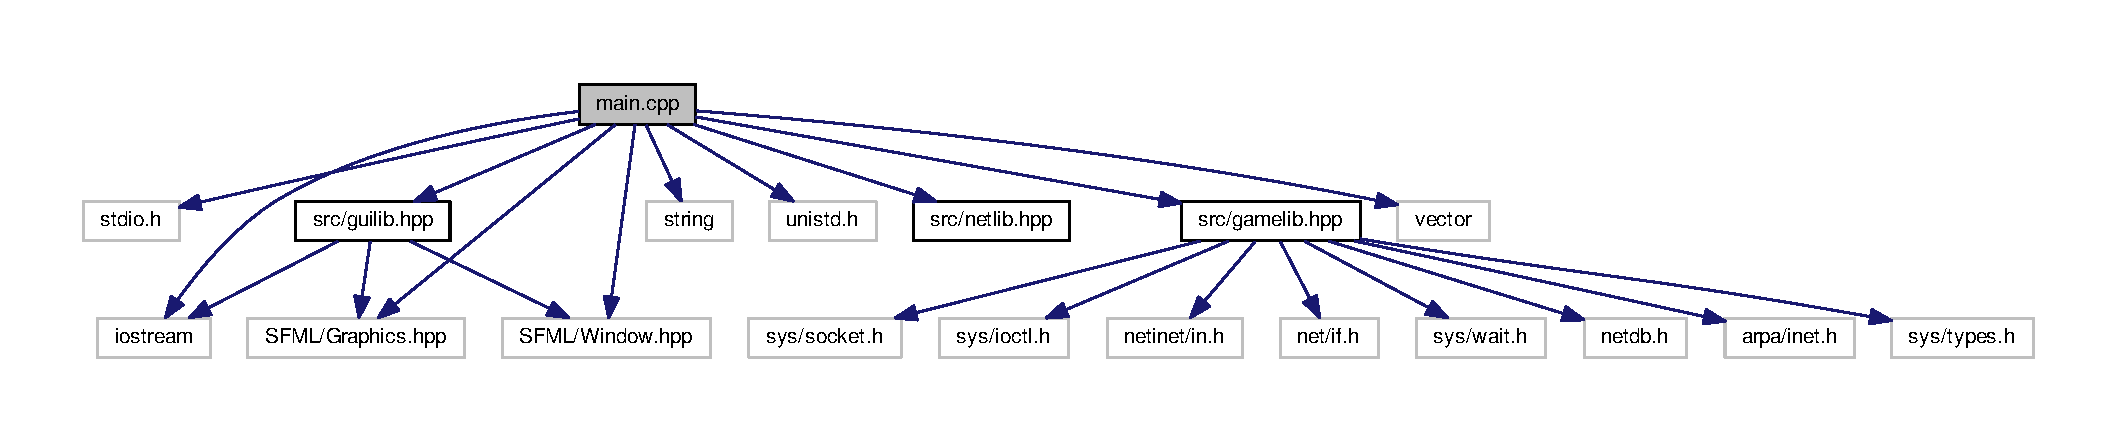
\includegraphics[width=350pt]{main_8cpp__incl}
\end{center}
\end{figure}
\subsection*{Functions}
\begin{DoxyCompactItemize}
\item 
int \hyperlink{main_8cpp_ae66f6b31b5ad750f1fe042a706a4e3d4}{main} ()
\end{DoxyCompactItemize}


\subsection{Function Documentation}
\index{main.\+cpp@{main.\+cpp}!main@{main}}
\index{main@{main}!main.\+cpp@{main.\+cpp}}
\subsubsection[{\texorpdfstring{main()}{main()}}]{\setlength{\rightskip}{0pt plus 5cm}int main (
\begin{DoxyParamCaption}
{}
\end{DoxyParamCaption}
)}\hypertarget{main_8cpp_ae66f6b31b5ad750f1fe042a706a4e3d4}{}\label{main_8cpp_ae66f6b31b5ad750f1fe042a706a4e3d4}

\hypertarget{gamelib_8cpp}{}\section{src/gamelib.cpp File Reference}
\label{gamelib_8cpp}\index{src/gamelib.\+cpp@{src/gamelib.\+cpp}}
{\ttfamily \#include $<$stdio.\+h$>$}\\*
{\ttfamily \#include $<$iostream$>$}\\*
{\ttfamily \#include $<$unistd.\+h$>$}\\*
{\ttfamily \#include $<$stdlib.\+h$>$}\\*
{\ttfamily \#include $<$string$>$}\\*
{\ttfamily \#include $<$string.\+h$>$}\\*
{\ttfamily \#include $<$S\+F\+M\+L/\+Graphics.\+hpp$>$}\\*
{\ttfamily \#include $<$S\+F\+M\+L/\+Window.\+hpp$>$}\\*
{\ttfamily \#include \char`\"{}netlib.\+hpp\char`\"{}}\\*
{\ttfamily \#include \char`\"{}guilib.\+hpp\char`\"{}}\\*
{\ttfamily \#include \char`\"{}gamelib.\+hpp\char`\"{}}\\*
{\ttfamily \#include \char`\"{}vector\char`\"{}}\\*
{\ttfamily \#include $<$sys/types.\+h$>$}\\*
{\ttfamily \#include $<$sys/socket.\+h$>$}\\*
{\ttfamily \#include $<$sys/ioctl.\+h$>$}\\*
{\ttfamily \#include $<$netinet/in.\+h$>$}\\*
{\ttfamily \#include $<$net/if.\+h$>$}\\*
{\ttfamily \#include $<$sys/wait.\+h$>$}\\*
{\ttfamily \#include $<$netdb.\+h$>$}\\*
{\ttfamily \#include $<$arpa/inet.\+h$>$}\\*
{\ttfamily \#include $<$fcntl.\+h$>$}\\*
{\ttfamily \#include $<$pthread.\+h$>$}\\*
Include dependency graph for gamelib.\+cpp\+:\nopagebreak
\begin{figure}[H]
\begin{center}
\leavevmode
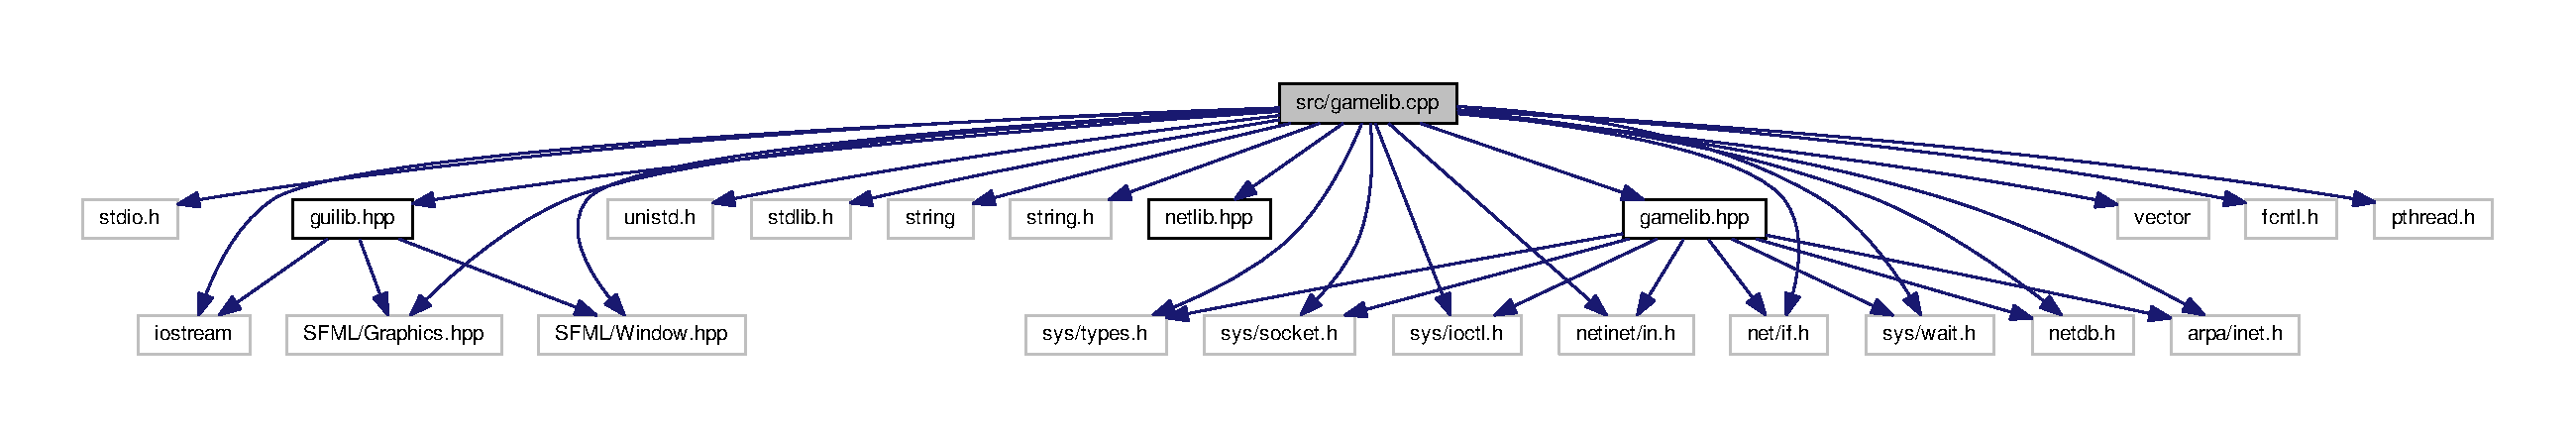
\includegraphics[width=350pt]{gamelib_8cpp__incl}
\end{center}
\end{figure}
\subsection*{Macros}
\begin{DoxyCompactItemize}
\item 
\#define \hyperlink{gamelib_8cpp_a82cd61d8dfabc6a7d9ab209995f85e93}{S\+E\+R\+V\+E\+R\+P\+O\+RT}~4000
\item 
\#define \hyperlink{gamelib_8cpp_a077fb1c484e71e2492507fa4459910ca}{W\+A\+T\+C\+H\+P\+O\+RT}~4001
\end{DoxyCompactItemize}


\subsection{Macro Definition Documentation}
\index{gamelib.\+cpp@{gamelib.\+cpp}!S\+E\+R\+V\+E\+R\+P\+O\+RT@{S\+E\+R\+V\+E\+R\+P\+O\+RT}}
\index{S\+E\+R\+V\+E\+R\+P\+O\+RT@{S\+E\+R\+V\+E\+R\+P\+O\+RT}!gamelib.\+cpp@{gamelib.\+cpp}}
\subsubsection[{\texorpdfstring{S\+E\+R\+V\+E\+R\+P\+O\+RT}{SERVERPORT}}]{\setlength{\rightskip}{0pt plus 5cm}\#define S\+E\+R\+V\+E\+R\+P\+O\+RT~4000}\hypertarget{gamelib_8cpp_a82cd61d8dfabc6a7d9ab209995f85e93}{}\label{gamelib_8cpp_a82cd61d8dfabc6a7d9ab209995f85e93}
\index{gamelib.\+cpp@{gamelib.\+cpp}!W\+A\+T\+C\+H\+P\+O\+RT@{W\+A\+T\+C\+H\+P\+O\+RT}}
\index{W\+A\+T\+C\+H\+P\+O\+RT@{W\+A\+T\+C\+H\+P\+O\+RT}!gamelib.\+cpp@{gamelib.\+cpp}}
\subsubsection[{\texorpdfstring{W\+A\+T\+C\+H\+P\+O\+RT}{WATCHPORT}}]{\setlength{\rightskip}{0pt plus 5cm}\#define W\+A\+T\+C\+H\+P\+O\+RT~4001}\hypertarget{gamelib_8cpp_a077fb1c484e71e2492507fa4459910ca}{}\label{gamelib_8cpp_a077fb1c484e71e2492507fa4459910ca}

\hypertarget{gamelib_8hpp}{}\section{src/gamelib.hpp File Reference}
\label{gamelib_8hpp}\index{src/gamelib.\+hpp@{src/gamelib.\+hpp}}
{\ttfamily \#include $<$sys/types.\+h$>$}\\*
{\ttfamily \#include $<$sys/socket.\+h$>$}\\*
{\ttfamily \#include $<$sys/ioctl.\+h$>$}\\*
{\ttfamily \#include $<$netinet/in.\+h$>$}\\*
{\ttfamily \#include $<$net/if.\+h$>$}\\*
{\ttfamily \#include $<$sys/wait.\+h$>$}\\*
{\ttfamily \#include $<$netdb.\+h$>$}\\*
{\ttfamily \#include $<$arpa/inet.\+h$>$}\\*
Include dependency graph for gamelib.\+hpp\+:\nopagebreak
\begin{figure}[H]
\begin{center}
\leavevmode
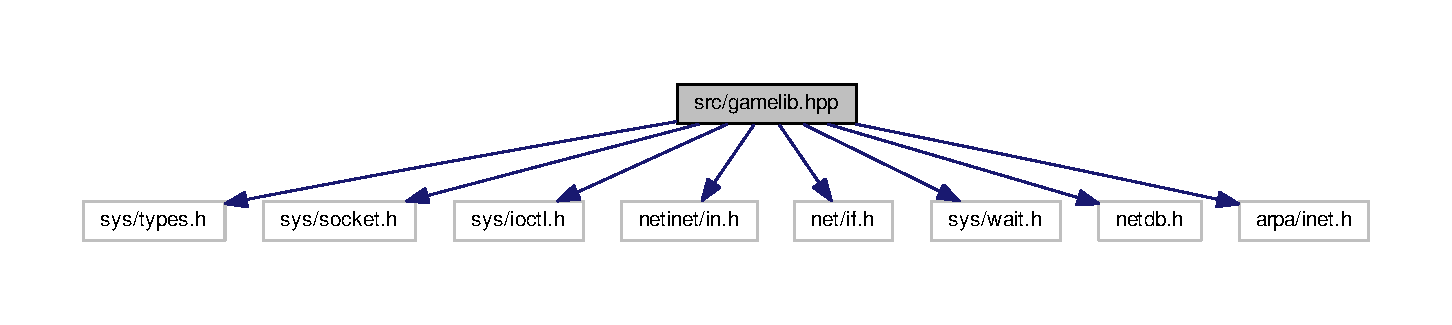
\includegraphics[width=350pt]{gamelib_8hpp__incl}
\end{center}
\end{figure}
This graph shows which files directly or indirectly include this file\+:\nopagebreak
\begin{figure}[H]
\begin{center}
\leavevmode
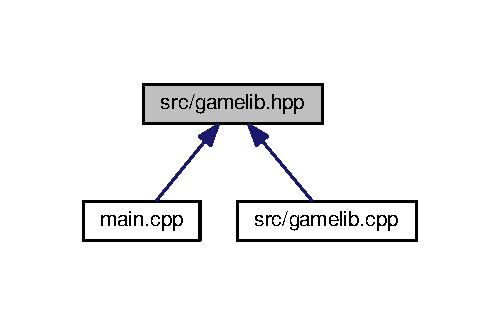
\includegraphics[width=240pt]{gamelib_8hpp__dep__incl}
\end{center}
\end{figure}
\subsection*{Classes}
\begin{DoxyCompactItemize}
\item 
struct \hyperlink{struct___player}{\+\_\+\+Player}
\item 
class \hyperlink{class_game}{Game}
\begin{DoxyCompactList}\small\item\em This class represent the game application. It owns the different methods running the game. \end{DoxyCompactList}\end{DoxyCompactItemize}
\subsection*{Macros}
\begin{DoxyCompactItemize}
\item 
\#define \hyperlink{gamelib_8hpp_a44dd1b46a3f55007e78fc1ac506153b9}{M\+A\+I\+N\+\_\+\+M\+E\+NU}~0
\item 
\#define \hyperlink{gamelib_8hpp_ac11b1add7fbae1e2fd3eb4db280e726e}{O\+P\+T\+I\+O\+N\+\_\+\+M\+E\+NU}~1
\item 
\#define \hyperlink{gamelib_8hpp_ad0f28d6602fd831f4b23b07600cb5663}{L\+A\+N\+\_\+\+M\+E\+NU}~2
\item 
\#define \hyperlink{gamelib_8hpp_ae4dc9aa573dd719b4e8d32de866a0676}{C\+R\+E\+A\+T\+I\+O\+N\+\_\+\+M\+E\+NU}~3
\item 
\#define \hyperlink{gamelib_8hpp_aac183cf41be6b5a75586c846e66fe880}{G\+A\+M\+E\+\_\+\+O\+N\+L\+I\+NE}~4
\item 
\#define \hyperlink{gamelib_8hpp_ae1fadc8bfc98bcc5f8283e1d266adbff}{M\+A\+I\+N\+\_\+\+G\+A\+ME}~5
\item 
\#define \hyperlink{gamelib_8hpp_a83e0919ddf2c586d3ed818dcff337a72}{I\+N\+Q\+U\+I\+R\+Y\+\_\+\+G\+A\+ME}~6
\item 
\#define \hyperlink{gamelib_8hpp_a08dd6ca7b9249fce702b62e83a83e257}{D\+E\+N\+O\+U\+N\+C\+E\+\_\+\+G\+A\+ME}~7
\item 
\#define \hyperlink{gamelib_8hpp_acffd6b8fc9934d27093805fb799425d6}{G\+E\+N\+P\+O\+L\+L\+\_\+\+G\+A\+ME}~8
\item 
\#define \hyperlink{gamelib_8hpp_aed7818555b2da57314243d796315e4e9}{G\+A\+M\+E\+\_\+\+N\+A\+ME}~\char`\"{}S\+H\+E\+R\+L\+O\+CK 13\char`\"{}
\item 
\#define \hyperlink{gamelib_8hpp_a23f7b870356588ddfcc49a1c364cba5e}{W\+I\+N\+\_\+W}~1200
\item 
\#define \hyperlink{gamelib_8hpp_ae893136b52eb3d95f3a310c3900ae42b}{W\+I\+N\+\_\+H}~700
\item 
\#define \hyperlink{gamelib_8hpp_add1d02207dbd9f34dd565662fb111e13}{G\+A\+M\+E\+\_\+\+F\+O\+N\+T\+\_\+\+T\+I\+T\+LE}~\char`\"{}media/fonts/S\+H\+E\+R\+L\+O\+C\+K\+E\+D.\+ttf\char`\"{}
\item 
\#define \hyperlink{gamelib_8hpp_aded335b4483d125c8bc278d8a01d71b3}{G\+A\+M\+E\+\_\+\+F\+O\+N\+T\+\_\+\+B\+U\+T\+T\+ON}~\char`\"{}media/fonts/S\+H\+E\+R\+L\+O\+C\+K\+E\+D.\+ttf\char`\"{}
\item 
\#define \hyperlink{gamelib_8hpp_ac4683d0496148f549de5e1c8565cfde4}{G\+A\+M\+E\+\_\+\+T\+H\+E\+M\+E\+\_\+\+B\+U\+T\+T\+ON}~\char`\"{}media/theme/button.\+png\char`\"{}
\item 
\#define \hyperlink{gamelib_8hpp_a2ffe207d8c7eafc9fc1dcf5847195288}{G\+A\+M\+E\+\_\+\+T\+H\+E\+M\+E\+\_\+\+A\+R\+R\+AY}~\char`\"{}media/theme/array\+Connection.\+png\char`\"{}
\item 
\#define \hyperlink{gamelib_8hpp_a430008b68b5b6c24d322a3aa655642e9}{L\+A\+N\+P\+O\+RT}~2027
\item 
\#define \hyperlink{gamelib_8hpp_a64bd201cde3669cc93407f6d8a50f8a0}{P\+L\+A\+Y\+\_\+\+B\+U\+TT}~1
\item 
\#define \hyperlink{gamelib_8hpp_a7cc616abbe656c9f94db9b129b1dbda3}{L\+A\+N\+\_\+\+B\+U\+TT}~2
\item 
\#define \hyperlink{gamelib_8hpp_a1d996f78877419ea4eaaccdd2f451f15}{O\+P\+T\+I\+O\+N\+\_\+\+B\+U\+TT}~3
\item 
\#define \hyperlink{gamelib_8hpp_a95bf13245b70fce1174ee9218f22d5d9}{Q\+U\+I\+T\+\_\+\+B\+U\+TT}~4
\item 
\#define \hyperlink{gamelib_8hpp_aab03d9ae79cbecdeb46c69fed8a60b82}{S\+A\+V\+E\+\_\+\+B\+U\+TT}~5
\item 
\#define \hyperlink{gamelib_8hpp_a2cc20321e1647892ae7c16c19e117c3d}{B\+A\+C\+K\+\_\+\+B\+U\+TT}~6
\item 
\#define \hyperlink{gamelib_8hpp_ab8b49e0cd147d6d52b467115e0bdb933}{H\+O\+S\+T\+\_\+\+B\+U\+TT}~7
\item 
\#define \hyperlink{gamelib_8hpp_a496dce15452e2878070951e95d3b8776}{J\+O\+I\+N\+\_\+\+B\+U\+TT}~8
\item 
\#define \hyperlink{gamelib_8hpp_a9815ff7e5dc007c4691dbbee06bafe72}{G\+E\+N\+P\+O\+L\+L\+\_\+\+B\+U\+TT}~9
\item 
\#define \hyperlink{gamelib_8hpp_af742ce1e9fe0a34a9924ddaf891984ec}{I\+N\+Q\+U\+I\+R\+Y\+\_\+\+B\+U\+TT}~10
\item 
\#define \hyperlink{gamelib_8hpp_aa0d8c9786802ff96d2fcc6d08000338f}{D\+E\+N\+O\+U\+N\+C\+E\+\_\+\+B\+U\+TT}~11
\item 
\#define \hyperlink{gamelib_8hpp_aa4bdd3d404ff4909adb7d4e503eb5f7a}{J\+E\+W\+E\+L\+R\+Y\+\_\+\+B\+U\+TT}~12
\item 
\#define \hyperlink{gamelib_8hpp_ade59382a2fdac955b24f5bbdccb31ab7}{B\+U\+L\+B\+\_\+\+B\+U\+TT}~13
\item 
\#define \hyperlink{gamelib_8hpp_ab2f73a6aedf9c55f56b710ebcf376658}{B\+O\+O\+K\+\_\+\+B\+U\+TT}~14
\item 
\#define \hyperlink{gamelib_8hpp_ac7b31119636771ed0c04654f311e1fe6}{M\+E\+D\+A\+L\+\_\+\+B\+U\+TT}~15
\item 
\#define \hyperlink{gamelib_8hpp_a104281d2d6d51838fd0cc6c0c430994a}{S\+K\+U\+L\+L\+\_\+\+B\+U\+TT}~16
\item 
\#define \hyperlink{gamelib_8hpp_a9dd909bcc2021f46c0b75fe756e935d0}{E\+Y\+E\+\_\+\+B\+U\+TT}~17
\item 
\#define \hyperlink{gamelib_8hpp_a9cb6cf5a477c18ac7164e30c6e13ddbc}{P\+I\+P\+E\+\_\+\+B\+U\+TT}~18
\item 
\#define \hyperlink{gamelib_8hpp_a47c75756ece46f6be55c7e257465dcea}{F\+I\+S\+T\+\_\+\+B\+U\+TT}~19
\item 
\#define \hyperlink{gamelib_8hpp_a1e77d39a04ce491a2e3d48f122d4cb6d}{S\+T\+A\+R\+T\+\_\+\+B\+U\+TT}~20
\item 
\#define \hyperlink{gamelib_8hpp_a9ea596e2bccc42c0b5d75191af5f7d97}{R\+E\+F\+R\+E\+S\+H\+\_\+\+B\+U\+TT}~25
\item 
\#define \hyperlink{gamelib_8hpp_a57531d535074e8e056c252093721c0c3}{K\+I\+L\+L\+\_\+\+P1\+\_\+\+B\+U\+TT}~21
\item 
\#define \hyperlink{gamelib_8hpp_af9535f703ec9e9bcc9422ad48c8c0290}{K\+I\+L\+L\+\_\+\+P2\+\_\+\+B\+U\+TT}~22
\item 
\#define \hyperlink{gamelib_8hpp_ac14297352497f9a5872d5f9b1aa40d03}{K\+I\+L\+L\+\_\+\+P3\+\_\+\+B\+U\+TT}~23
\item 
\#define \hyperlink{gamelib_8hpp_a4c731403ae9f4cff5835eb323491eb03}{K\+I\+L\+L\+\_\+\+P4\+\_\+\+B\+U\+TT}~24
\item 
\#define \hyperlink{gamelib_8hpp_a3131502d495aa5b9b94f46522fd4a783}{J\+O\+I\+N\+\_\+\+S1\+\_\+\+B\+U\+TT}~31
\item 
\#define \hyperlink{gamelib_8hpp_ac12679eb63170b2a934f198b7506bfe1}{J\+O\+I\+N\+\_\+\+S2\+\_\+\+B\+U\+TT}~32
\item 
\#define \hyperlink{gamelib_8hpp_a934ef4fd3d746e009562c07e645391d9}{J\+O\+I\+N\+\_\+\+S3\+\_\+\+B\+U\+TT}~33
\item 
\#define \hyperlink{gamelib_8hpp_a427b8fdb6813d998aaeaac911472439c}{J\+O\+I\+N\+\_\+\+S4\+\_\+\+B\+U\+TT}~34
\item 
\#define \hyperlink{gamelib_8hpp_a4e075bf3de224196253c911045648e71}{N\+B\+\_\+\+O\+BJ}~8
\item 
\#define \hyperlink{gamelib_8hpp_af247743e348b5c28e17999f4502b527c}{N\+B\+\_\+\+M\+A\+X\+\_\+\+P\+L\+A\+Y\+E\+RS}~4
\end{DoxyCompactItemize}
\subsection*{Typedefs}
\begin{DoxyCompactItemize}
\item 
typedef struct \hyperlink{struct___player}{\+\_\+\+Player} \hyperlink{gamelib_8hpp_af30e2030635a69690f85e48bc6ef202f}{Player}
\end{DoxyCompactItemize}


\subsection{Macro Definition Documentation}
\index{gamelib.\+hpp@{gamelib.\+hpp}!B\+A\+C\+K\+\_\+\+B\+U\+TT@{B\+A\+C\+K\+\_\+\+B\+U\+TT}}
\index{B\+A\+C\+K\+\_\+\+B\+U\+TT@{B\+A\+C\+K\+\_\+\+B\+U\+TT}!gamelib.\+hpp@{gamelib.\+hpp}}
\subsubsection[{\texorpdfstring{B\+A\+C\+K\+\_\+\+B\+U\+TT}{BACK_BUTT}}]{\setlength{\rightskip}{0pt plus 5cm}\#define B\+A\+C\+K\+\_\+\+B\+U\+TT~6}\hypertarget{gamelib_8hpp_a2cc20321e1647892ae7c16c19e117c3d}{}\label{gamelib_8hpp_a2cc20321e1647892ae7c16c19e117c3d}
\index{gamelib.\+hpp@{gamelib.\+hpp}!B\+O\+O\+K\+\_\+\+B\+U\+TT@{B\+O\+O\+K\+\_\+\+B\+U\+TT}}
\index{B\+O\+O\+K\+\_\+\+B\+U\+TT@{B\+O\+O\+K\+\_\+\+B\+U\+TT}!gamelib.\+hpp@{gamelib.\+hpp}}
\subsubsection[{\texorpdfstring{B\+O\+O\+K\+\_\+\+B\+U\+TT}{BOOK_BUTT}}]{\setlength{\rightskip}{0pt plus 5cm}\#define B\+O\+O\+K\+\_\+\+B\+U\+TT~14}\hypertarget{gamelib_8hpp_ab2f73a6aedf9c55f56b710ebcf376658}{}\label{gamelib_8hpp_ab2f73a6aedf9c55f56b710ebcf376658}
\index{gamelib.\+hpp@{gamelib.\+hpp}!B\+U\+L\+B\+\_\+\+B\+U\+TT@{B\+U\+L\+B\+\_\+\+B\+U\+TT}}
\index{B\+U\+L\+B\+\_\+\+B\+U\+TT@{B\+U\+L\+B\+\_\+\+B\+U\+TT}!gamelib.\+hpp@{gamelib.\+hpp}}
\subsubsection[{\texorpdfstring{B\+U\+L\+B\+\_\+\+B\+U\+TT}{BULB_BUTT}}]{\setlength{\rightskip}{0pt plus 5cm}\#define B\+U\+L\+B\+\_\+\+B\+U\+TT~13}\hypertarget{gamelib_8hpp_ade59382a2fdac955b24f5bbdccb31ab7}{}\label{gamelib_8hpp_ade59382a2fdac955b24f5bbdccb31ab7}
\index{gamelib.\+hpp@{gamelib.\+hpp}!C\+R\+E\+A\+T\+I\+O\+N\+\_\+\+M\+E\+NU@{C\+R\+E\+A\+T\+I\+O\+N\+\_\+\+M\+E\+NU}}
\index{C\+R\+E\+A\+T\+I\+O\+N\+\_\+\+M\+E\+NU@{C\+R\+E\+A\+T\+I\+O\+N\+\_\+\+M\+E\+NU}!gamelib.\+hpp@{gamelib.\+hpp}}
\subsubsection[{\texorpdfstring{C\+R\+E\+A\+T\+I\+O\+N\+\_\+\+M\+E\+NU}{CREATION_MENU}}]{\setlength{\rightskip}{0pt plus 5cm}\#define C\+R\+E\+A\+T\+I\+O\+N\+\_\+\+M\+E\+NU~3}\hypertarget{gamelib_8hpp_ae4dc9aa573dd719b4e8d32de866a0676}{}\label{gamelib_8hpp_ae4dc9aa573dd719b4e8d32de866a0676}
\index{gamelib.\+hpp@{gamelib.\+hpp}!D\+E\+N\+O\+U\+N\+C\+E\+\_\+\+B\+U\+TT@{D\+E\+N\+O\+U\+N\+C\+E\+\_\+\+B\+U\+TT}}
\index{D\+E\+N\+O\+U\+N\+C\+E\+\_\+\+B\+U\+TT@{D\+E\+N\+O\+U\+N\+C\+E\+\_\+\+B\+U\+TT}!gamelib.\+hpp@{gamelib.\+hpp}}
\subsubsection[{\texorpdfstring{D\+E\+N\+O\+U\+N\+C\+E\+\_\+\+B\+U\+TT}{DENOUNCE_BUTT}}]{\setlength{\rightskip}{0pt plus 5cm}\#define D\+E\+N\+O\+U\+N\+C\+E\+\_\+\+B\+U\+TT~11}\hypertarget{gamelib_8hpp_aa0d8c9786802ff96d2fcc6d08000338f}{}\label{gamelib_8hpp_aa0d8c9786802ff96d2fcc6d08000338f}
\index{gamelib.\+hpp@{gamelib.\+hpp}!D\+E\+N\+O\+U\+N\+C\+E\+\_\+\+G\+A\+ME@{D\+E\+N\+O\+U\+N\+C\+E\+\_\+\+G\+A\+ME}}
\index{D\+E\+N\+O\+U\+N\+C\+E\+\_\+\+G\+A\+ME@{D\+E\+N\+O\+U\+N\+C\+E\+\_\+\+G\+A\+ME}!gamelib.\+hpp@{gamelib.\+hpp}}
\subsubsection[{\texorpdfstring{D\+E\+N\+O\+U\+N\+C\+E\+\_\+\+G\+A\+ME}{DENOUNCE_GAME}}]{\setlength{\rightskip}{0pt plus 5cm}\#define D\+E\+N\+O\+U\+N\+C\+E\+\_\+\+G\+A\+ME~7}\hypertarget{gamelib_8hpp_a08dd6ca7b9249fce702b62e83a83e257}{}\label{gamelib_8hpp_a08dd6ca7b9249fce702b62e83a83e257}
\index{gamelib.\+hpp@{gamelib.\+hpp}!E\+Y\+E\+\_\+\+B\+U\+TT@{E\+Y\+E\+\_\+\+B\+U\+TT}}
\index{E\+Y\+E\+\_\+\+B\+U\+TT@{E\+Y\+E\+\_\+\+B\+U\+TT}!gamelib.\+hpp@{gamelib.\+hpp}}
\subsubsection[{\texorpdfstring{E\+Y\+E\+\_\+\+B\+U\+TT}{EYE_BUTT}}]{\setlength{\rightskip}{0pt plus 5cm}\#define E\+Y\+E\+\_\+\+B\+U\+TT~17}\hypertarget{gamelib_8hpp_a9dd909bcc2021f46c0b75fe756e935d0}{}\label{gamelib_8hpp_a9dd909bcc2021f46c0b75fe756e935d0}
\index{gamelib.\+hpp@{gamelib.\+hpp}!F\+I\+S\+T\+\_\+\+B\+U\+TT@{F\+I\+S\+T\+\_\+\+B\+U\+TT}}
\index{F\+I\+S\+T\+\_\+\+B\+U\+TT@{F\+I\+S\+T\+\_\+\+B\+U\+TT}!gamelib.\+hpp@{gamelib.\+hpp}}
\subsubsection[{\texorpdfstring{F\+I\+S\+T\+\_\+\+B\+U\+TT}{FIST_BUTT}}]{\setlength{\rightskip}{0pt plus 5cm}\#define F\+I\+S\+T\+\_\+\+B\+U\+TT~19}\hypertarget{gamelib_8hpp_a47c75756ece46f6be55c7e257465dcea}{}\label{gamelib_8hpp_a47c75756ece46f6be55c7e257465dcea}
\index{gamelib.\+hpp@{gamelib.\+hpp}!G\+A\+M\+E\+\_\+\+F\+O\+N\+T\+\_\+\+B\+U\+T\+T\+ON@{G\+A\+M\+E\+\_\+\+F\+O\+N\+T\+\_\+\+B\+U\+T\+T\+ON}}
\index{G\+A\+M\+E\+\_\+\+F\+O\+N\+T\+\_\+\+B\+U\+T\+T\+ON@{G\+A\+M\+E\+\_\+\+F\+O\+N\+T\+\_\+\+B\+U\+T\+T\+ON}!gamelib.\+hpp@{gamelib.\+hpp}}
\subsubsection[{\texorpdfstring{G\+A\+M\+E\+\_\+\+F\+O\+N\+T\+\_\+\+B\+U\+T\+T\+ON}{GAME_FONT_BUTTON}}]{\setlength{\rightskip}{0pt plus 5cm}\#define G\+A\+M\+E\+\_\+\+F\+O\+N\+T\+\_\+\+B\+U\+T\+T\+ON~\char`\"{}media/fonts/S\+H\+E\+R\+L\+O\+C\+K\+E\+D.\+ttf\char`\"{}}\hypertarget{gamelib_8hpp_aded335b4483d125c8bc278d8a01d71b3}{}\label{gamelib_8hpp_aded335b4483d125c8bc278d8a01d71b3}
\index{gamelib.\+hpp@{gamelib.\+hpp}!G\+A\+M\+E\+\_\+\+F\+O\+N\+T\+\_\+\+T\+I\+T\+LE@{G\+A\+M\+E\+\_\+\+F\+O\+N\+T\+\_\+\+T\+I\+T\+LE}}
\index{G\+A\+M\+E\+\_\+\+F\+O\+N\+T\+\_\+\+T\+I\+T\+LE@{G\+A\+M\+E\+\_\+\+F\+O\+N\+T\+\_\+\+T\+I\+T\+LE}!gamelib.\+hpp@{gamelib.\+hpp}}
\subsubsection[{\texorpdfstring{G\+A\+M\+E\+\_\+\+F\+O\+N\+T\+\_\+\+T\+I\+T\+LE}{GAME_FONT_TITLE}}]{\setlength{\rightskip}{0pt plus 5cm}\#define G\+A\+M\+E\+\_\+\+F\+O\+N\+T\+\_\+\+T\+I\+T\+LE~\char`\"{}media/fonts/S\+H\+E\+R\+L\+O\+C\+K\+E\+D.\+ttf\char`\"{}}\hypertarget{gamelib_8hpp_add1d02207dbd9f34dd565662fb111e13}{}\label{gamelib_8hpp_add1d02207dbd9f34dd565662fb111e13}
\index{gamelib.\+hpp@{gamelib.\+hpp}!G\+A\+M\+E\+\_\+\+N\+A\+ME@{G\+A\+M\+E\+\_\+\+N\+A\+ME}}
\index{G\+A\+M\+E\+\_\+\+N\+A\+ME@{G\+A\+M\+E\+\_\+\+N\+A\+ME}!gamelib.\+hpp@{gamelib.\+hpp}}
\subsubsection[{\texorpdfstring{G\+A\+M\+E\+\_\+\+N\+A\+ME}{GAME_NAME}}]{\setlength{\rightskip}{0pt plus 5cm}\#define G\+A\+M\+E\+\_\+\+N\+A\+ME~\char`\"{}S\+H\+E\+R\+L\+O\+CK 13\char`\"{}}\hypertarget{gamelib_8hpp_aed7818555b2da57314243d796315e4e9}{}\label{gamelib_8hpp_aed7818555b2da57314243d796315e4e9}
\index{gamelib.\+hpp@{gamelib.\+hpp}!G\+A\+M\+E\+\_\+\+O\+N\+L\+I\+NE@{G\+A\+M\+E\+\_\+\+O\+N\+L\+I\+NE}}
\index{G\+A\+M\+E\+\_\+\+O\+N\+L\+I\+NE@{G\+A\+M\+E\+\_\+\+O\+N\+L\+I\+NE}!gamelib.\+hpp@{gamelib.\+hpp}}
\subsubsection[{\texorpdfstring{G\+A\+M\+E\+\_\+\+O\+N\+L\+I\+NE}{GAME_ONLINE}}]{\setlength{\rightskip}{0pt plus 5cm}\#define G\+A\+M\+E\+\_\+\+O\+N\+L\+I\+NE~4}\hypertarget{gamelib_8hpp_aac183cf41be6b5a75586c846e66fe880}{}\label{gamelib_8hpp_aac183cf41be6b5a75586c846e66fe880}
\index{gamelib.\+hpp@{gamelib.\+hpp}!G\+A\+M\+E\+\_\+\+T\+H\+E\+M\+E\+\_\+\+A\+R\+R\+AY@{G\+A\+M\+E\+\_\+\+T\+H\+E\+M\+E\+\_\+\+A\+R\+R\+AY}}
\index{G\+A\+M\+E\+\_\+\+T\+H\+E\+M\+E\+\_\+\+A\+R\+R\+AY@{G\+A\+M\+E\+\_\+\+T\+H\+E\+M\+E\+\_\+\+A\+R\+R\+AY}!gamelib.\+hpp@{gamelib.\+hpp}}
\subsubsection[{\texorpdfstring{G\+A\+M\+E\+\_\+\+T\+H\+E\+M\+E\+\_\+\+A\+R\+R\+AY}{GAME_THEME_ARRAY}}]{\setlength{\rightskip}{0pt plus 5cm}\#define G\+A\+M\+E\+\_\+\+T\+H\+E\+M\+E\+\_\+\+A\+R\+R\+AY~\char`\"{}media/theme/array\+Connection.\+png\char`\"{}}\hypertarget{gamelib_8hpp_a2ffe207d8c7eafc9fc1dcf5847195288}{}\label{gamelib_8hpp_a2ffe207d8c7eafc9fc1dcf5847195288}
\index{gamelib.\+hpp@{gamelib.\+hpp}!G\+A\+M\+E\+\_\+\+T\+H\+E\+M\+E\+\_\+\+B\+U\+T\+T\+ON@{G\+A\+M\+E\+\_\+\+T\+H\+E\+M\+E\+\_\+\+B\+U\+T\+T\+ON}}
\index{G\+A\+M\+E\+\_\+\+T\+H\+E\+M\+E\+\_\+\+B\+U\+T\+T\+ON@{G\+A\+M\+E\+\_\+\+T\+H\+E\+M\+E\+\_\+\+B\+U\+T\+T\+ON}!gamelib.\+hpp@{gamelib.\+hpp}}
\subsubsection[{\texorpdfstring{G\+A\+M\+E\+\_\+\+T\+H\+E\+M\+E\+\_\+\+B\+U\+T\+T\+ON}{GAME_THEME_BUTTON}}]{\setlength{\rightskip}{0pt plus 5cm}\#define G\+A\+M\+E\+\_\+\+T\+H\+E\+M\+E\+\_\+\+B\+U\+T\+T\+ON~\char`\"{}media/theme/button.\+png\char`\"{}}\hypertarget{gamelib_8hpp_ac4683d0496148f549de5e1c8565cfde4}{}\label{gamelib_8hpp_ac4683d0496148f549de5e1c8565cfde4}
\index{gamelib.\+hpp@{gamelib.\+hpp}!G\+E\+N\+P\+O\+L\+L\+\_\+\+B\+U\+TT@{G\+E\+N\+P\+O\+L\+L\+\_\+\+B\+U\+TT}}
\index{G\+E\+N\+P\+O\+L\+L\+\_\+\+B\+U\+TT@{G\+E\+N\+P\+O\+L\+L\+\_\+\+B\+U\+TT}!gamelib.\+hpp@{gamelib.\+hpp}}
\subsubsection[{\texorpdfstring{G\+E\+N\+P\+O\+L\+L\+\_\+\+B\+U\+TT}{GENPOLL_BUTT}}]{\setlength{\rightskip}{0pt plus 5cm}\#define G\+E\+N\+P\+O\+L\+L\+\_\+\+B\+U\+TT~9}\hypertarget{gamelib_8hpp_a9815ff7e5dc007c4691dbbee06bafe72}{}\label{gamelib_8hpp_a9815ff7e5dc007c4691dbbee06bafe72}
\index{gamelib.\+hpp@{gamelib.\+hpp}!G\+E\+N\+P\+O\+L\+L\+\_\+\+G\+A\+ME@{G\+E\+N\+P\+O\+L\+L\+\_\+\+G\+A\+ME}}
\index{G\+E\+N\+P\+O\+L\+L\+\_\+\+G\+A\+ME@{G\+E\+N\+P\+O\+L\+L\+\_\+\+G\+A\+ME}!gamelib.\+hpp@{gamelib.\+hpp}}
\subsubsection[{\texorpdfstring{G\+E\+N\+P\+O\+L\+L\+\_\+\+G\+A\+ME}{GENPOLL_GAME}}]{\setlength{\rightskip}{0pt plus 5cm}\#define G\+E\+N\+P\+O\+L\+L\+\_\+\+G\+A\+ME~8}\hypertarget{gamelib_8hpp_acffd6b8fc9934d27093805fb799425d6}{}\label{gamelib_8hpp_acffd6b8fc9934d27093805fb799425d6}
\index{gamelib.\+hpp@{gamelib.\+hpp}!H\+O\+S\+T\+\_\+\+B\+U\+TT@{H\+O\+S\+T\+\_\+\+B\+U\+TT}}
\index{H\+O\+S\+T\+\_\+\+B\+U\+TT@{H\+O\+S\+T\+\_\+\+B\+U\+TT}!gamelib.\+hpp@{gamelib.\+hpp}}
\subsubsection[{\texorpdfstring{H\+O\+S\+T\+\_\+\+B\+U\+TT}{HOST_BUTT}}]{\setlength{\rightskip}{0pt plus 5cm}\#define H\+O\+S\+T\+\_\+\+B\+U\+TT~7}\hypertarget{gamelib_8hpp_ab8b49e0cd147d6d52b467115e0bdb933}{}\label{gamelib_8hpp_ab8b49e0cd147d6d52b467115e0bdb933}
\index{gamelib.\+hpp@{gamelib.\+hpp}!I\+N\+Q\+U\+I\+R\+Y\+\_\+\+B\+U\+TT@{I\+N\+Q\+U\+I\+R\+Y\+\_\+\+B\+U\+TT}}
\index{I\+N\+Q\+U\+I\+R\+Y\+\_\+\+B\+U\+TT@{I\+N\+Q\+U\+I\+R\+Y\+\_\+\+B\+U\+TT}!gamelib.\+hpp@{gamelib.\+hpp}}
\subsubsection[{\texorpdfstring{I\+N\+Q\+U\+I\+R\+Y\+\_\+\+B\+U\+TT}{INQUIRY_BUTT}}]{\setlength{\rightskip}{0pt plus 5cm}\#define I\+N\+Q\+U\+I\+R\+Y\+\_\+\+B\+U\+TT~10}\hypertarget{gamelib_8hpp_af742ce1e9fe0a34a9924ddaf891984ec}{}\label{gamelib_8hpp_af742ce1e9fe0a34a9924ddaf891984ec}
\index{gamelib.\+hpp@{gamelib.\+hpp}!I\+N\+Q\+U\+I\+R\+Y\+\_\+\+G\+A\+ME@{I\+N\+Q\+U\+I\+R\+Y\+\_\+\+G\+A\+ME}}
\index{I\+N\+Q\+U\+I\+R\+Y\+\_\+\+G\+A\+ME@{I\+N\+Q\+U\+I\+R\+Y\+\_\+\+G\+A\+ME}!gamelib.\+hpp@{gamelib.\+hpp}}
\subsubsection[{\texorpdfstring{I\+N\+Q\+U\+I\+R\+Y\+\_\+\+G\+A\+ME}{INQUIRY_GAME}}]{\setlength{\rightskip}{0pt plus 5cm}\#define I\+N\+Q\+U\+I\+R\+Y\+\_\+\+G\+A\+ME~6}\hypertarget{gamelib_8hpp_a83e0919ddf2c586d3ed818dcff337a72}{}\label{gamelib_8hpp_a83e0919ddf2c586d3ed818dcff337a72}
\index{gamelib.\+hpp@{gamelib.\+hpp}!J\+E\+W\+E\+L\+R\+Y\+\_\+\+B\+U\+TT@{J\+E\+W\+E\+L\+R\+Y\+\_\+\+B\+U\+TT}}
\index{J\+E\+W\+E\+L\+R\+Y\+\_\+\+B\+U\+TT@{J\+E\+W\+E\+L\+R\+Y\+\_\+\+B\+U\+TT}!gamelib.\+hpp@{gamelib.\+hpp}}
\subsubsection[{\texorpdfstring{J\+E\+W\+E\+L\+R\+Y\+\_\+\+B\+U\+TT}{JEWELRY_BUTT}}]{\setlength{\rightskip}{0pt plus 5cm}\#define J\+E\+W\+E\+L\+R\+Y\+\_\+\+B\+U\+TT~12}\hypertarget{gamelib_8hpp_aa4bdd3d404ff4909adb7d4e503eb5f7a}{}\label{gamelib_8hpp_aa4bdd3d404ff4909adb7d4e503eb5f7a}
\index{gamelib.\+hpp@{gamelib.\+hpp}!J\+O\+I\+N\+\_\+\+B\+U\+TT@{J\+O\+I\+N\+\_\+\+B\+U\+TT}}
\index{J\+O\+I\+N\+\_\+\+B\+U\+TT@{J\+O\+I\+N\+\_\+\+B\+U\+TT}!gamelib.\+hpp@{gamelib.\+hpp}}
\subsubsection[{\texorpdfstring{J\+O\+I\+N\+\_\+\+B\+U\+TT}{JOIN_BUTT}}]{\setlength{\rightskip}{0pt plus 5cm}\#define J\+O\+I\+N\+\_\+\+B\+U\+TT~8}\hypertarget{gamelib_8hpp_a496dce15452e2878070951e95d3b8776}{}\label{gamelib_8hpp_a496dce15452e2878070951e95d3b8776}
\index{gamelib.\+hpp@{gamelib.\+hpp}!J\+O\+I\+N\+\_\+\+S1\+\_\+\+B\+U\+TT@{J\+O\+I\+N\+\_\+\+S1\+\_\+\+B\+U\+TT}}
\index{J\+O\+I\+N\+\_\+\+S1\+\_\+\+B\+U\+TT@{J\+O\+I\+N\+\_\+\+S1\+\_\+\+B\+U\+TT}!gamelib.\+hpp@{gamelib.\+hpp}}
\subsubsection[{\texorpdfstring{J\+O\+I\+N\+\_\+\+S1\+\_\+\+B\+U\+TT}{JOIN_S1_BUTT}}]{\setlength{\rightskip}{0pt plus 5cm}\#define J\+O\+I\+N\+\_\+\+S1\+\_\+\+B\+U\+TT~31}\hypertarget{gamelib_8hpp_a3131502d495aa5b9b94f46522fd4a783}{}\label{gamelib_8hpp_a3131502d495aa5b9b94f46522fd4a783}
\index{gamelib.\+hpp@{gamelib.\+hpp}!J\+O\+I\+N\+\_\+\+S2\+\_\+\+B\+U\+TT@{J\+O\+I\+N\+\_\+\+S2\+\_\+\+B\+U\+TT}}
\index{J\+O\+I\+N\+\_\+\+S2\+\_\+\+B\+U\+TT@{J\+O\+I\+N\+\_\+\+S2\+\_\+\+B\+U\+TT}!gamelib.\+hpp@{gamelib.\+hpp}}
\subsubsection[{\texorpdfstring{J\+O\+I\+N\+\_\+\+S2\+\_\+\+B\+U\+TT}{JOIN_S2_BUTT}}]{\setlength{\rightskip}{0pt plus 5cm}\#define J\+O\+I\+N\+\_\+\+S2\+\_\+\+B\+U\+TT~32}\hypertarget{gamelib_8hpp_ac12679eb63170b2a934f198b7506bfe1}{}\label{gamelib_8hpp_ac12679eb63170b2a934f198b7506bfe1}
\index{gamelib.\+hpp@{gamelib.\+hpp}!J\+O\+I\+N\+\_\+\+S3\+\_\+\+B\+U\+TT@{J\+O\+I\+N\+\_\+\+S3\+\_\+\+B\+U\+TT}}
\index{J\+O\+I\+N\+\_\+\+S3\+\_\+\+B\+U\+TT@{J\+O\+I\+N\+\_\+\+S3\+\_\+\+B\+U\+TT}!gamelib.\+hpp@{gamelib.\+hpp}}
\subsubsection[{\texorpdfstring{J\+O\+I\+N\+\_\+\+S3\+\_\+\+B\+U\+TT}{JOIN_S3_BUTT}}]{\setlength{\rightskip}{0pt plus 5cm}\#define J\+O\+I\+N\+\_\+\+S3\+\_\+\+B\+U\+TT~33}\hypertarget{gamelib_8hpp_a934ef4fd3d746e009562c07e645391d9}{}\label{gamelib_8hpp_a934ef4fd3d746e009562c07e645391d9}
\index{gamelib.\+hpp@{gamelib.\+hpp}!J\+O\+I\+N\+\_\+\+S4\+\_\+\+B\+U\+TT@{J\+O\+I\+N\+\_\+\+S4\+\_\+\+B\+U\+TT}}
\index{J\+O\+I\+N\+\_\+\+S4\+\_\+\+B\+U\+TT@{J\+O\+I\+N\+\_\+\+S4\+\_\+\+B\+U\+TT}!gamelib.\+hpp@{gamelib.\+hpp}}
\subsubsection[{\texorpdfstring{J\+O\+I\+N\+\_\+\+S4\+\_\+\+B\+U\+TT}{JOIN_S4_BUTT}}]{\setlength{\rightskip}{0pt plus 5cm}\#define J\+O\+I\+N\+\_\+\+S4\+\_\+\+B\+U\+TT~34}\hypertarget{gamelib_8hpp_a427b8fdb6813d998aaeaac911472439c}{}\label{gamelib_8hpp_a427b8fdb6813d998aaeaac911472439c}
\index{gamelib.\+hpp@{gamelib.\+hpp}!K\+I\+L\+L\+\_\+\+P1\+\_\+\+B\+U\+TT@{K\+I\+L\+L\+\_\+\+P1\+\_\+\+B\+U\+TT}}
\index{K\+I\+L\+L\+\_\+\+P1\+\_\+\+B\+U\+TT@{K\+I\+L\+L\+\_\+\+P1\+\_\+\+B\+U\+TT}!gamelib.\+hpp@{gamelib.\+hpp}}
\subsubsection[{\texorpdfstring{K\+I\+L\+L\+\_\+\+P1\+\_\+\+B\+U\+TT}{KILL_P1_BUTT}}]{\setlength{\rightskip}{0pt plus 5cm}\#define K\+I\+L\+L\+\_\+\+P1\+\_\+\+B\+U\+TT~21}\hypertarget{gamelib_8hpp_a57531d535074e8e056c252093721c0c3}{}\label{gamelib_8hpp_a57531d535074e8e056c252093721c0c3}
\index{gamelib.\+hpp@{gamelib.\+hpp}!K\+I\+L\+L\+\_\+\+P2\+\_\+\+B\+U\+TT@{K\+I\+L\+L\+\_\+\+P2\+\_\+\+B\+U\+TT}}
\index{K\+I\+L\+L\+\_\+\+P2\+\_\+\+B\+U\+TT@{K\+I\+L\+L\+\_\+\+P2\+\_\+\+B\+U\+TT}!gamelib.\+hpp@{gamelib.\+hpp}}
\subsubsection[{\texorpdfstring{K\+I\+L\+L\+\_\+\+P2\+\_\+\+B\+U\+TT}{KILL_P2_BUTT}}]{\setlength{\rightskip}{0pt plus 5cm}\#define K\+I\+L\+L\+\_\+\+P2\+\_\+\+B\+U\+TT~22}\hypertarget{gamelib_8hpp_af9535f703ec9e9bcc9422ad48c8c0290}{}\label{gamelib_8hpp_af9535f703ec9e9bcc9422ad48c8c0290}
\index{gamelib.\+hpp@{gamelib.\+hpp}!K\+I\+L\+L\+\_\+\+P3\+\_\+\+B\+U\+TT@{K\+I\+L\+L\+\_\+\+P3\+\_\+\+B\+U\+TT}}
\index{K\+I\+L\+L\+\_\+\+P3\+\_\+\+B\+U\+TT@{K\+I\+L\+L\+\_\+\+P3\+\_\+\+B\+U\+TT}!gamelib.\+hpp@{gamelib.\+hpp}}
\subsubsection[{\texorpdfstring{K\+I\+L\+L\+\_\+\+P3\+\_\+\+B\+U\+TT}{KILL_P3_BUTT}}]{\setlength{\rightskip}{0pt plus 5cm}\#define K\+I\+L\+L\+\_\+\+P3\+\_\+\+B\+U\+TT~23}\hypertarget{gamelib_8hpp_ac14297352497f9a5872d5f9b1aa40d03}{}\label{gamelib_8hpp_ac14297352497f9a5872d5f9b1aa40d03}
\index{gamelib.\+hpp@{gamelib.\+hpp}!K\+I\+L\+L\+\_\+\+P4\+\_\+\+B\+U\+TT@{K\+I\+L\+L\+\_\+\+P4\+\_\+\+B\+U\+TT}}
\index{K\+I\+L\+L\+\_\+\+P4\+\_\+\+B\+U\+TT@{K\+I\+L\+L\+\_\+\+P4\+\_\+\+B\+U\+TT}!gamelib.\+hpp@{gamelib.\+hpp}}
\subsubsection[{\texorpdfstring{K\+I\+L\+L\+\_\+\+P4\+\_\+\+B\+U\+TT}{KILL_P4_BUTT}}]{\setlength{\rightskip}{0pt plus 5cm}\#define K\+I\+L\+L\+\_\+\+P4\+\_\+\+B\+U\+TT~24}\hypertarget{gamelib_8hpp_a4c731403ae9f4cff5835eb323491eb03}{}\label{gamelib_8hpp_a4c731403ae9f4cff5835eb323491eb03}
\index{gamelib.\+hpp@{gamelib.\+hpp}!L\+A\+N\+\_\+\+B\+U\+TT@{L\+A\+N\+\_\+\+B\+U\+TT}}
\index{L\+A\+N\+\_\+\+B\+U\+TT@{L\+A\+N\+\_\+\+B\+U\+TT}!gamelib.\+hpp@{gamelib.\+hpp}}
\subsubsection[{\texorpdfstring{L\+A\+N\+\_\+\+B\+U\+TT}{LAN_BUTT}}]{\setlength{\rightskip}{0pt plus 5cm}\#define L\+A\+N\+\_\+\+B\+U\+TT~2}\hypertarget{gamelib_8hpp_a7cc616abbe656c9f94db9b129b1dbda3}{}\label{gamelib_8hpp_a7cc616abbe656c9f94db9b129b1dbda3}
\index{gamelib.\+hpp@{gamelib.\+hpp}!L\+A\+N\+\_\+\+M\+E\+NU@{L\+A\+N\+\_\+\+M\+E\+NU}}
\index{L\+A\+N\+\_\+\+M\+E\+NU@{L\+A\+N\+\_\+\+M\+E\+NU}!gamelib.\+hpp@{gamelib.\+hpp}}
\subsubsection[{\texorpdfstring{L\+A\+N\+\_\+\+M\+E\+NU}{LAN_MENU}}]{\setlength{\rightskip}{0pt plus 5cm}\#define L\+A\+N\+\_\+\+M\+E\+NU~2}\hypertarget{gamelib_8hpp_ad0f28d6602fd831f4b23b07600cb5663}{}\label{gamelib_8hpp_ad0f28d6602fd831f4b23b07600cb5663}
\index{gamelib.\+hpp@{gamelib.\+hpp}!L\+A\+N\+P\+O\+RT@{L\+A\+N\+P\+O\+RT}}
\index{L\+A\+N\+P\+O\+RT@{L\+A\+N\+P\+O\+RT}!gamelib.\+hpp@{gamelib.\+hpp}}
\subsubsection[{\texorpdfstring{L\+A\+N\+P\+O\+RT}{LANPORT}}]{\setlength{\rightskip}{0pt plus 5cm}\#define L\+A\+N\+P\+O\+RT~2027}\hypertarget{gamelib_8hpp_a430008b68b5b6c24d322a3aa655642e9}{}\label{gamelib_8hpp_a430008b68b5b6c24d322a3aa655642e9}
\index{gamelib.\+hpp@{gamelib.\+hpp}!M\+A\+I\+N\+\_\+\+G\+A\+ME@{M\+A\+I\+N\+\_\+\+G\+A\+ME}}
\index{M\+A\+I\+N\+\_\+\+G\+A\+ME@{M\+A\+I\+N\+\_\+\+G\+A\+ME}!gamelib.\+hpp@{gamelib.\+hpp}}
\subsubsection[{\texorpdfstring{M\+A\+I\+N\+\_\+\+G\+A\+ME}{MAIN_GAME}}]{\setlength{\rightskip}{0pt plus 5cm}\#define M\+A\+I\+N\+\_\+\+G\+A\+ME~5}\hypertarget{gamelib_8hpp_ae1fadc8bfc98bcc5f8283e1d266adbff}{}\label{gamelib_8hpp_ae1fadc8bfc98bcc5f8283e1d266adbff}
\index{gamelib.\+hpp@{gamelib.\+hpp}!M\+A\+I\+N\+\_\+\+M\+E\+NU@{M\+A\+I\+N\+\_\+\+M\+E\+NU}}
\index{M\+A\+I\+N\+\_\+\+M\+E\+NU@{M\+A\+I\+N\+\_\+\+M\+E\+NU}!gamelib.\+hpp@{gamelib.\+hpp}}
\subsubsection[{\texorpdfstring{M\+A\+I\+N\+\_\+\+M\+E\+NU}{MAIN_MENU}}]{\setlength{\rightskip}{0pt plus 5cm}\#define M\+A\+I\+N\+\_\+\+M\+E\+NU~0}\hypertarget{gamelib_8hpp_a44dd1b46a3f55007e78fc1ac506153b9}{}\label{gamelib_8hpp_a44dd1b46a3f55007e78fc1ac506153b9}
\index{gamelib.\+hpp@{gamelib.\+hpp}!M\+E\+D\+A\+L\+\_\+\+B\+U\+TT@{M\+E\+D\+A\+L\+\_\+\+B\+U\+TT}}
\index{M\+E\+D\+A\+L\+\_\+\+B\+U\+TT@{M\+E\+D\+A\+L\+\_\+\+B\+U\+TT}!gamelib.\+hpp@{gamelib.\+hpp}}
\subsubsection[{\texorpdfstring{M\+E\+D\+A\+L\+\_\+\+B\+U\+TT}{MEDAL_BUTT}}]{\setlength{\rightskip}{0pt plus 5cm}\#define M\+E\+D\+A\+L\+\_\+\+B\+U\+TT~15}\hypertarget{gamelib_8hpp_ac7b31119636771ed0c04654f311e1fe6}{}\label{gamelib_8hpp_ac7b31119636771ed0c04654f311e1fe6}
\index{gamelib.\+hpp@{gamelib.\+hpp}!N\+B\+\_\+\+M\+A\+X\+\_\+\+P\+L\+A\+Y\+E\+RS@{N\+B\+\_\+\+M\+A\+X\+\_\+\+P\+L\+A\+Y\+E\+RS}}
\index{N\+B\+\_\+\+M\+A\+X\+\_\+\+P\+L\+A\+Y\+E\+RS@{N\+B\+\_\+\+M\+A\+X\+\_\+\+P\+L\+A\+Y\+E\+RS}!gamelib.\+hpp@{gamelib.\+hpp}}
\subsubsection[{\texorpdfstring{N\+B\+\_\+\+M\+A\+X\+\_\+\+P\+L\+A\+Y\+E\+RS}{NB_MAX_PLAYERS}}]{\setlength{\rightskip}{0pt plus 5cm}\#define N\+B\+\_\+\+M\+A\+X\+\_\+\+P\+L\+A\+Y\+E\+RS~4}\hypertarget{gamelib_8hpp_af247743e348b5c28e17999f4502b527c}{}\label{gamelib_8hpp_af247743e348b5c28e17999f4502b527c}
\index{gamelib.\+hpp@{gamelib.\+hpp}!N\+B\+\_\+\+O\+BJ@{N\+B\+\_\+\+O\+BJ}}
\index{N\+B\+\_\+\+O\+BJ@{N\+B\+\_\+\+O\+BJ}!gamelib.\+hpp@{gamelib.\+hpp}}
\subsubsection[{\texorpdfstring{N\+B\+\_\+\+O\+BJ}{NB_OBJ}}]{\setlength{\rightskip}{0pt plus 5cm}\#define N\+B\+\_\+\+O\+BJ~8}\hypertarget{gamelib_8hpp_a4e075bf3de224196253c911045648e71}{}\label{gamelib_8hpp_a4e075bf3de224196253c911045648e71}
\index{gamelib.\+hpp@{gamelib.\+hpp}!O\+P\+T\+I\+O\+N\+\_\+\+B\+U\+TT@{O\+P\+T\+I\+O\+N\+\_\+\+B\+U\+TT}}
\index{O\+P\+T\+I\+O\+N\+\_\+\+B\+U\+TT@{O\+P\+T\+I\+O\+N\+\_\+\+B\+U\+TT}!gamelib.\+hpp@{gamelib.\+hpp}}
\subsubsection[{\texorpdfstring{O\+P\+T\+I\+O\+N\+\_\+\+B\+U\+TT}{OPTION_BUTT}}]{\setlength{\rightskip}{0pt plus 5cm}\#define O\+P\+T\+I\+O\+N\+\_\+\+B\+U\+TT~3}\hypertarget{gamelib_8hpp_a1d996f78877419ea4eaaccdd2f451f15}{}\label{gamelib_8hpp_a1d996f78877419ea4eaaccdd2f451f15}
\index{gamelib.\+hpp@{gamelib.\+hpp}!O\+P\+T\+I\+O\+N\+\_\+\+M\+E\+NU@{O\+P\+T\+I\+O\+N\+\_\+\+M\+E\+NU}}
\index{O\+P\+T\+I\+O\+N\+\_\+\+M\+E\+NU@{O\+P\+T\+I\+O\+N\+\_\+\+M\+E\+NU}!gamelib.\+hpp@{gamelib.\+hpp}}
\subsubsection[{\texorpdfstring{O\+P\+T\+I\+O\+N\+\_\+\+M\+E\+NU}{OPTION_MENU}}]{\setlength{\rightskip}{0pt plus 5cm}\#define O\+P\+T\+I\+O\+N\+\_\+\+M\+E\+NU~1}\hypertarget{gamelib_8hpp_ac11b1add7fbae1e2fd3eb4db280e726e}{}\label{gamelib_8hpp_ac11b1add7fbae1e2fd3eb4db280e726e}
\index{gamelib.\+hpp@{gamelib.\+hpp}!P\+I\+P\+E\+\_\+\+B\+U\+TT@{P\+I\+P\+E\+\_\+\+B\+U\+TT}}
\index{P\+I\+P\+E\+\_\+\+B\+U\+TT@{P\+I\+P\+E\+\_\+\+B\+U\+TT}!gamelib.\+hpp@{gamelib.\+hpp}}
\subsubsection[{\texorpdfstring{P\+I\+P\+E\+\_\+\+B\+U\+TT}{PIPE_BUTT}}]{\setlength{\rightskip}{0pt plus 5cm}\#define P\+I\+P\+E\+\_\+\+B\+U\+TT~18}\hypertarget{gamelib_8hpp_a9cb6cf5a477c18ac7164e30c6e13ddbc}{}\label{gamelib_8hpp_a9cb6cf5a477c18ac7164e30c6e13ddbc}
\index{gamelib.\+hpp@{gamelib.\+hpp}!P\+L\+A\+Y\+\_\+\+B\+U\+TT@{P\+L\+A\+Y\+\_\+\+B\+U\+TT}}
\index{P\+L\+A\+Y\+\_\+\+B\+U\+TT@{P\+L\+A\+Y\+\_\+\+B\+U\+TT}!gamelib.\+hpp@{gamelib.\+hpp}}
\subsubsection[{\texorpdfstring{P\+L\+A\+Y\+\_\+\+B\+U\+TT}{PLAY_BUTT}}]{\setlength{\rightskip}{0pt plus 5cm}\#define P\+L\+A\+Y\+\_\+\+B\+U\+TT~1}\hypertarget{gamelib_8hpp_a64bd201cde3669cc93407f6d8a50f8a0}{}\label{gamelib_8hpp_a64bd201cde3669cc93407f6d8a50f8a0}
\index{gamelib.\+hpp@{gamelib.\+hpp}!Q\+U\+I\+T\+\_\+\+B\+U\+TT@{Q\+U\+I\+T\+\_\+\+B\+U\+TT}}
\index{Q\+U\+I\+T\+\_\+\+B\+U\+TT@{Q\+U\+I\+T\+\_\+\+B\+U\+TT}!gamelib.\+hpp@{gamelib.\+hpp}}
\subsubsection[{\texorpdfstring{Q\+U\+I\+T\+\_\+\+B\+U\+TT}{QUIT_BUTT}}]{\setlength{\rightskip}{0pt plus 5cm}\#define Q\+U\+I\+T\+\_\+\+B\+U\+TT~4}\hypertarget{gamelib_8hpp_a95bf13245b70fce1174ee9218f22d5d9}{}\label{gamelib_8hpp_a95bf13245b70fce1174ee9218f22d5d9}
\index{gamelib.\+hpp@{gamelib.\+hpp}!R\+E\+F\+R\+E\+S\+H\+\_\+\+B\+U\+TT@{R\+E\+F\+R\+E\+S\+H\+\_\+\+B\+U\+TT}}
\index{R\+E\+F\+R\+E\+S\+H\+\_\+\+B\+U\+TT@{R\+E\+F\+R\+E\+S\+H\+\_\+\+B\+U\+TT}!gamelib.\+hpp@{gamelib.\+hpp}}
\subsubsection[{\texorpdfstring{R\+E\+F\+R\+E\+S\+H\+\_\+\+B\+U\+TT}{REFRESH_BUTT}}]{\setlength{\rightskip}{0pt plus 5cm}\#define R\+E\+F\+R\+E\+S\+H\+\_\+\+B\+U\+TT~25}\hypertarget{gamelib_8hpp_a9ea596e2bccc42c0b5d75191af5f7d97}{}\label{gamelib_8hpp_a9ea596e2bccc42c0b5d75191af5f7d97}
\index{gamelib.\+hpp@{gamelib.\+hpp}!S\+A\+V\+E\+\_\+\+B\+U\+TT@{S\+A\+V\+E\+\_\+\+B\+U\+TT}}
\index{S\+A\+V\+E\+\_\+\+B\+U\+TT@{S\+A\+V\+E\+\_\+\+B\+U\+TT}!gamelib.\+hpp@{gamelib.\+hpp}}
\subsubsection[{\texorpdfstring{S\+A\+V\+E\+\_\+\+B\+U\+TT}{SAVE_BUTT}}]{\setlength{\rightskip}{0pt plus 5cm}\#define S\+A\+V\+E\+\_\+\+B\+U\+TT~5}\hypertarget{gamelib_8hpp_aab03d9ae79cbecdeb46c69fed8a60b82}{}\label{gamelib_8hpp_aab03d9ae79cbecdeb46c69fed8a60b82}
\index{gamelib.\+hpp@{gamelib.\+hpp}!S\+K\+U\+L\+L\+\_\+\+B\+U\+TT@{S\+K\+U\+L\+L\+\_\+\+B\+U\+TT}}
\index{S\+K\+U\+L\+L\+\_\+\+B\+U\+TT@{S\+K\+U\+L\+L\+\_\+\+B\+U\+TT}!gamelib.\+hpp@{gamelib.\+hpp}}
\subsubsection[{\texorpdfstring{S\+K\+U\+L\+L\+\_\+\+B\+U\+TT}{SKULL_BUTT}}]{\setlength{\rightskip}{0pt plus 5cm}\#define S\+K\+U\+L\+L\+\_\+\+B\+U\+TT~16}\hypertarget{gamelib_8hpp_a104281d2d6d51838fd0cc6c0c430994a}{}\label{gamelib_8hpp_a104281d2d6d51838fd0cc6c0c430994a}
\index{gamelib.\+hpp@{gamelib.\+hpp}!S\+T\+A\+R\+T\+\_\+\+B\+U\+TT@{S\+T\+A\+R\+T\+\_\+\+B\+U\+TT}}
\index{S\+T\+A\+R\+T\+\_\+\+B\+U\+TT@{S\+T\+A\+R\+T\+\_\+\+B\+U\+TT}!gamelib.\+hpp@{gamelib.\+hpp}}
\subsubsection[{\texorpdfstring{S\+T\+A\+R\+T\+\_\+\+B\+U\+TT}{START_BUTT}}]{\setlength{\rightskip}{0pt plus 5cm}\#define S\+T\+A\+R\+T\+\_\+\+B\+U\+TT~20}\hypertarget{gamelib_8hpp_a1e77d39a04ce491a2e3d48f122d4cb6d}{}\label{gamelib_8hpp_a1e77d39a04ce491a2e3d48f122d4cb6d}
\index{gamelib.\+hpp@{gamelib.\+hpp}!W\+I\+N\+\_\+H@{W\+I\+N\+\_\+H}}
\index{W\+I\+N\+\_\+H@{W\+I\+N\+\_\+H}!gamelib.\+hpp@{gamelib.\+hpp}}
\subsubsection[{\texorpdfstring{W\+I\+N\+\_\+H}{WIN_H}}]{\setlength{\rightskip}{0pt plus 5cm}\#define W\+I\+N\+\_\+H~700}\hypertarget{gamelib_8hpp_ae893136b52eb3d95f3a310c3900ae42b}{}\label{gamelib_8hpp_ae893136b52eb3d95f3a310c3900ae42b}
\index{gamelib.\+hpp@{gamelib.\+hpp}!W\+I\+N\+\_\+W@{W\+I\+N\+\_\+W}}
\index{W\+I\+N\+\_\+W@{W\+I\+N\+\_\+W}!gamelib.\+hpp@{gamelib.\+hpp}}
\subsubsection[{\texorpdfstring{W\+I\+N\+\_\+W}{WIN_W}}]{\setlength{\rightskip}{0pt plus 5cm}\#define W\+I\+N\+\_\+W~1200}\hypertarget{gamelib_8hpp_a23f7b870356588ddfcc49a1c364cba5e}{}\label{gamelib_8hpp_a23f7b870356588ddfcc49a1c364cba5e}


\subsection{Typedef Documentation}
\index{gamelib.\+hpp@{gamelib.\+hpp}!Player@{Player}}
\index{Player@{Player}!gamelib.\+hpp@{gamelib.\+hpp}}
\subsubsection[{\texorpdfstring{Player}{Player}}]{\setlength{\rightskip}{0pt plus 5cm}typedef struct {\bf \+\_\+\+Player} {\bf Player}}\hypertarget{gamelib_8hpp_af30e2030635a69690f85e48bc6ef202f}{}\label{gamelib_8hpp_af30e2030635a69690f85e48bc6ef202f}

\hypertarget{guilib_8cpp}{}\section{src/guilib.cpp File Reference}
\label{guilib_8cpp}\index{src/guilib.\+cpp@{src/guilib.\+cpp}}
{\ttfamily \#include \char`\"{}guilib.\+hpp\char`\"{}}\\*
{\ttfamily \#include $<$stdio.\+h$>$}\\*
Include dependency graph for guilib.\+cpp\+:\nopagebreak
\begin{figure}[H]
\begin{center}
\leavevmode
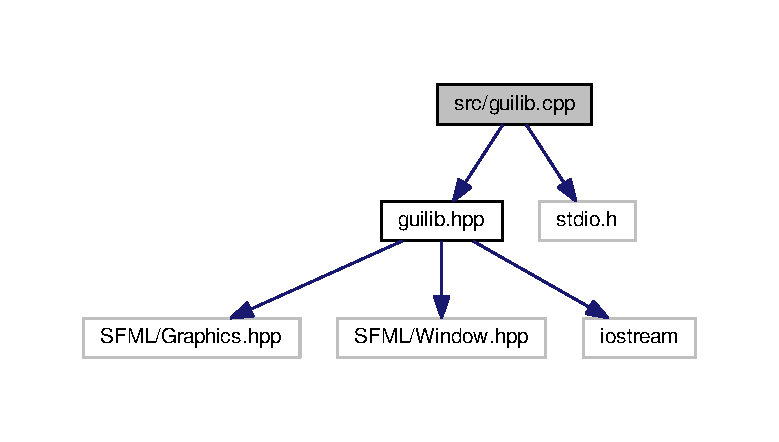
\includegraphics[width=350pt]{guilib_8cpp__incl}
\end{center}
\end{figure}

\hypertarget{guilib_8hpp}{}\section{src/guilib.hpp File Reference}
\label{guilib_8hpp}\index{src/guilib.\+hpp@{src/guilib.\+hpp}}
{\ttfamily \#include $<$S\+F\+M\+L/\+Graphics.\+hpp$>$}\\*
{\ttfamily \#include $<$S\+F\+M\+L/\+Window.\+hpp$>$}\\*
{\ttfamily \#include $<$iostream$>$}\\*
Include dependency graph for guilib.\+hpp\+:\nopagebreak
\begin{figure}[H]
\begin{center}
\leavevmode
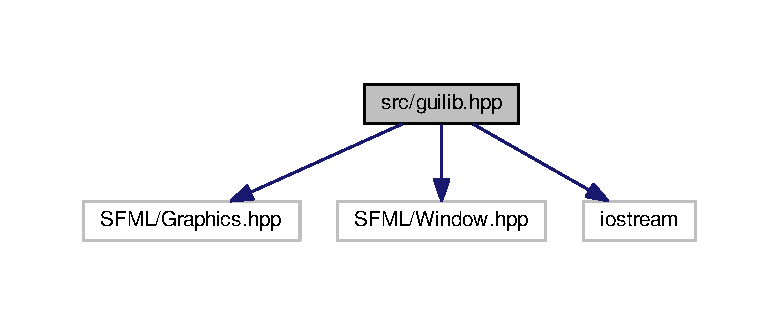
\includegraphics[width=350pt]{guilib_8hpp__incl}
\end{center}
\end{figure}
This graph shows which files directly or indirectly include this file\+:\nopagebreak
\begin{figure}[H]
\begin{center}
\leavevmode
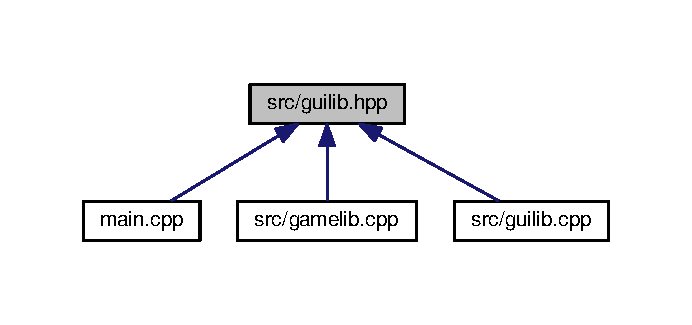
\includegraphics[width=332pt]{guilib_8hpp__dep__incl}
\end{center}
\end{figure}
\subsection*{Classes}
\begin{DoxyCompactItemize}
\item 
class \hyperlink{class_button}{Button}
\item 
class \hyperlink{class_textbox}{Textbox}
\end{DoxyCompactItemize}

\hypertarget{netlib_8cpp}{}\section{src/netlib.cpp File Reference}
\label{netlib_8cpp}\index{src/netlib.\+cpp@{src/netlib.\+cpp}}
{\ttfamily \#include $<$stdio.\+h$>$}\\*
{\ttfamily \#include $<$stdlib.\+h$>$}\\*
{\ttfamily \#include $<$string.\+h$>$}\\*
{\ttfamily \#include $<$unistd.\+h$>$}\\*
{\ttfamily \#include $<$sys/types.\+h$>$}\\*
{\ttfamily \#include $<$sys/socket.\+h$>$}\\*
{\ttfamily \#include $<$netinet/in.\+h$>$}\\*
{\ttfamily \#include $<$netdb.\+h$>$}\\*
{\ttfamily \#include $<$arpa/inet.\+h$>$}\\*
{\ttfamily \#include $<$sys/ioctl.\+h$>$}\\*
{\ttfamily \#include $<$net/if.\+h$>$}\\*
{\ttfamily \#include $<$sys/wait.\+h$>$}\\*
{\ttfamily \#include $<$fcntl.\+h$>$}\\*
{\ttfamily \#include \char`\"{}netlib.\+hpp\char`\"{}}\\*
{\ttfamily \#include $<$err.\+h$>$}\\*
{\ttfamily \#include $<$errno.\+h$>$}\\*
{\ttfamily \#include \char`\"{}vector\char`\"{}}\\*
{\ttfamily \#include $<$iostream$>$}\\*
Include dependency graph for netlib.\+cpp\+:\nopagebreak
\begin{figure}[H]
\begin{center}
\leavevmode
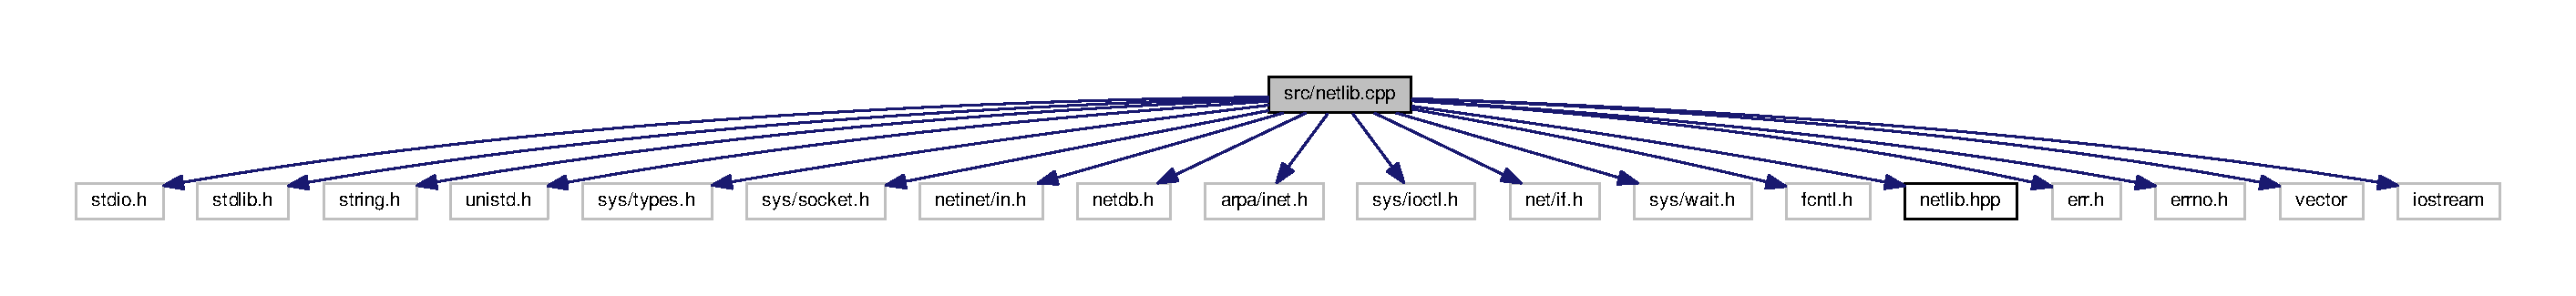
\includegraphics[width=350pt]{netlib_8cpp__incl}
\end{center}
\end{figure}
\subsection*{Functions}
\begin{DoxyCompactItemize}
\item 
int \hyperlink{netlib_8cpp_a09d73a7c513d94589e8150ea2df254b7}{send\+T\+CP} (const char $\ast$I\+Paddress, int port, \hyperlink{netlib_8hpp_a2e50028ebd48ce86d5b1fc983d6ef155}{Buffer} $\ast$buff)
\item 
int \hyperlink{netlib_8cpp_ab73c457f96397f02201e8124c8493377}{scan\+Servers} (\hyperlink{netlib_8hpp_a95e7ffbda40674e59bb208b9c6c9a22a}{Server} servers\mbox{[}5\mbox{]})
\begin{DoxyCompactList}\small\item\em Scan the different IP address and store the servers sh13 found inside the servers array passed in argument. \end{DoxyCompactList}\end{DoxyCompactItemize}


\subsection{Function Documentation}
\index{netlib.\+cpp@{netlib.\+cpp}!scan\+Servers@{scan\+Servers}}
\index{scan\+Servers@{scan\+Servers}!netlib.\+cpp@{netlib.\+cpp}}
\subsubsection[{\texorpdfstring{scan\+Servers(\+Server servers[5])}{scanServers(Server servers[5])}}]{\setlength{\rightskip}{0pt plus 5cm}scan\+Servers (
\begin{DoxyParamCaption}
\item[{{\bf Server}}]{servers\mbox{[}5\mbox{]}}
\end{DoxyParamCaption}
)}\hypertarget{netlib_8cpp_ab73c457f96397f02201e8124c8493377}{}\label{netlib_8cpp_ab73c457f96397f02201e8124c8493377}


Scan the different IP address and store the servers sh13 found inside the servers array passed in argument. 


\begin{DoxyParams}{Parameters}
{\em server\mbox{[}5\mbox{]}} & Arrays of servers found. \\
\hline
\end{DoxyParams}
\index{netlib.\+cpp@{netlib.\+cpp}!send\+T\+CP@{send\+T\+CP}}
\index{send\+T\+CP@{send\+T\+CP}!netlib.\+cpp@{netlib.\+cpp}}
\subsubsection[{\texorpdfstring{send\+T\+C\+P(const char $\ast$\+I\+Paddress, int port, Buffer $\ast$buff)}{sendTCP(const char *IPaddress, int port, Buffer *buff)}}]{\setlength{\rightskip}{0pt plus 5cm}int send\+T\+CP (
\begin{DoxyParamCaption}
\item[{const char $\ast$}]{I\+Paddress, }
\item[{int}]{port, }
\item[{{\bf Buffer} $\ast$}]{buff}
\end{DoxyParamCaption}
)}\hypertarget{netlib_8cpp_a09d73a7c513d94589e8150ea2df254b7}{}\label{netlib_8cpp_a09d73a7c513d94589e8150ea2df254b7}

\hypertarget{netlib_8hpp}{}\section{src/netlib.hpp File Reference}
\label{netlib_8hpp}\index{src/netlib.\+hpp@{src/netlib.\+hpp}}
This graph shows which files directly or indirectly include this file\+:\nopagebreak
\begin{figure}[H]
\begin{center}
\leavevmode
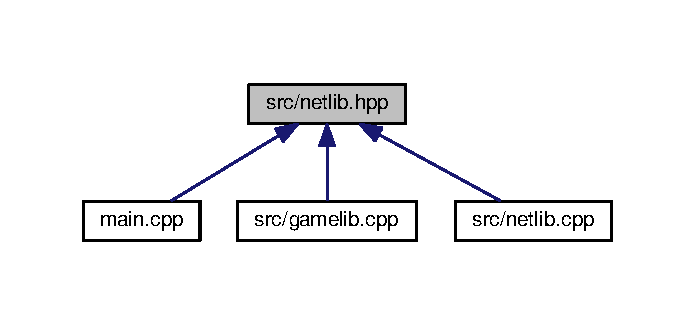
\includegraphics[width=334pt]{netlib_8hpp__dep__incl}
\end{center}
\end{figure}
\subsection*{Classes}
\begin{DoxyCompactItemize}
\item 
struct \hyperlink{struct___buffer}{\+\_\+\+Buffer}
\begin{DoxyCompactList}\small\item\em Structures of transmission and reception buffers. \end{DoxyCompactList}\item 
struct \hyperlink{struct___server}{\+\_\+\+Server}
\begin{DoxyCompactList}\small\item\em Structure of different data link to severs. \end{DoxyCompactList}\end{DoxyCompactItemize}
\subsection*{Macros}
\begin{DoxyCompactItemize}
\item 
\#define \hyperlink{netlib_8hpp_afecd0d3dfa9d17ffdc75f686ea643d9b}{S\+I\+Z\+E\+\_\+\+B\+U\+FF}~256
\end{DoxyCompactItemize}
\subsection*{Typedefs}
\begin{DoxyCompactItemize}
\item 
typedef struct \hyperlink{struct___buffer}{\+\_\+\+Buffer} \hyperlink{netlib_8hpp_a2e50028ebd48ce86d5b1fc983d6ef155}{Buffer}
\item 
typedef struct \hyperlink{struct___server}{\+\_\+\+Server} \hyperlink{netlib_8hpp_a95e7ffbda40674e59bb208b9c6c9a22a}{Server}
\end{DoxyCompactItemize}
\subsection*{Functions}
\begin{DoxyCompactItemize}
\item 
int \hyperlink{netlib_8hpp_a09d73a7c513d94589e8150ea2df254b7}{send\+T\+CP} (const char $\ast$I\+Paddress, int port, \hyperlink{netlib_8hpp_a2e50028ebd48ce86d5b1fc983d6ef155}{Buffer} $\ast$buff)
\item 
int \hyperlink{netlib_8hpp_ade29426fa34f49349dee2ac58b2cfeef}{scan\+Servers} (\hyperlink{netlib_8hpp_a95e7ffbda40674e59bb208b9c6c9a22a}{Server} servers\mbox{[}5\mbox{]})
\begin{DoxyCompactList}\small\item\em Scan the different IP address and store the servers sh13 found inside the servers array passed in argument. \end{DoxyCompactList}\end{DoxyCompactItemize}


\subsection{Macro Definition Documentation}
\index{netlib.\+hpp@{netlib.\+hpp}!S\+I\+Z\+E\+\_\+\+B\+U\+FF@{S\+I\+Z\+E\+\_\+\+B\+U\+FF}}
\index{S\+I\+Z\+E\+\_\+\+B\+U\+FF@{S\+I\+Z\+E\+\_\+\+B\+U\+FF}!netlib.\+hpp@{netlib.\+hpp}}
\subsubsection[{\texorpdfstring{S\+I\+Z\+E\+\_\+\+B\+U\+FF}{SIZE_BUFF}}]{\setlength{\rightskip}{0pt plus 5cm}\#define S\+I\+Z\+E\+\_\+\+B\+U\+FF~256}\hypertarget{netlib_8hpp_afecd0d3dfa9d17ffdc75f686ea643d9b}{}\label{netlib_8hpp_afecd0d3dfa9d17ffdc75f686ea643d9b}


\subsection{Typedef Documentation}
\index{netlib.\+hpp@{netlib.\+hpp}!Buffer@{Buffer}}
\index{Buffer@{Buffer}!netlib.\+hpp@{netlib.\+hpp}}
\subsubsection[{\texorpdfstring{Buffer}{Buffer}}]{\setlength{\rightskip}{0pt plus 5cm}typedef struct {\bf \+\_\+\+Buffer} {\bf Buffer}}\hypertarget{netlib_8hpp_a2e50028ebd48ce86d5b1fc983d6ef155}{}\label{netlib_8hpp_a2e50028ebd48ce86d5b1fc983d6ef155}
\index{netlib.\+hpp@{netlib.\+hpp}!Server@{Server}}
\index{Server@{Server}!netlib.\+hpp@{netlib.\+hpp}}
\subsubsection[{\texorpdfstring{Server}{Server}}]{\setlength{\rightskip}{0pt plus 5cm}typedef struct {\bf \+\_\+\+Server} {\bf Server}}\hypertarget{netlib_8hpp_a95e7ffbda40674e59bb208b9c6c9a22a}{}\label{netlib_8hpp_a95e7ffbda40674e59bb208b9c6c9a22a}


\subsection{Function Documentation}
\index{netlib.\+hpp@{netlib.\+hpp}!scan\+Servers@{scan\+Servers}}
\index{scan\+Servers@{scan\+Servers}!netlib.\+hpp@{netlib.\+hpp}}
\subsubsection[{\texorpdfstring{scan\+Servers(\+Server servers[5])}{scanServers(Server servers[5])}}]{\setlength{\rightskip}{0pt plus 5cm}int scan\+Servers (
\begin{DoxyParamCaption}
\item[{{\bf Server}}]{servers\mbox{[}5\mbox{]}}
\end{DoxyParamCaption}
)}\hypertarget{netlib_8hpp_ade29426fa34f49349dee2ac58b2cfeef}{}\label{netlib_8hpp_ade29426fa34f49349dee2ac58b2cfeef}


Scan the different IP address and store the servers sh13 found inside the servers array passed in argument. 


\begin{DoxyParams}{Parameters}
{\em server\mbox{[}5\mbox{]}} & Arrays of servers found. \\
\hline
\end{DoxyParams}
\index{netlib.\+hpp@{netlib.\+hpp}!send\+T\+CP@{send\+T\+CP}}
\index{send\+T\+CP@{send\+T\+CP}!netlib.\+hpp@{netlib.\+hpp}}
\subsubsection[{\texorpdfstring{send\+T\+C\+P(const char $\ast$\+I\+Paddress, int port, Buffer $\ast$buff)}{sendTCP(const char *IPaddress, int port, Buffer *buff)}}]{\setlength{\rightskip}{0pt plus 5cm}int send\+T\+CP (
\begin{DoxyParamCaption}
\item[{const char $\ast$}]{I\+Paddress, }
\item[{int}]{port, }
\item[{{\bf Buffer} $\ast$}]{buff}
\end{DoxyParamCaption}
)}\hypertarget{netlib_8hpp_a09d73a7c513d94589e8150ea2df254b7}{}\label{netlib_8hpp_a09d73a7c513d94589e8150ea2df254b7}

%--- End generated contents ---

% Index
\backmatter
\newpage
\phantomsection
\clearemptydoublepage
\addcontentsline{toc}{chapter}{Index}
\printindex

\end{document}
